\documentclass{article}
\usepackage[utf8]{inputenc}

\usepackage{parskip}
\setlength{\parskip}{\baselineskip}%
\setlength{\parindent}{0pt}%

\usepackage{enumitem}
\setlist{nosep} % or \setlist{noitemsep} to leave space around whole list

\usepackage[normalem]{ulem}

\usepackage{fourier} 
\usepackage{array}
\usepackage{makecell}

\renewcommand\theadalign{bc}
\renewcommand\theadfont{\bfseries}
\renewcommand\theadgape{\Gape[4pt]}
\renewcommand\cellgape{\Gape[4pt]}

\usepackage[
backend=biber,
style=authoryear,
citestyle=authoryear,
maxbibnames=99,
uniquelist=false,
natbib=true
]{biblatex}
\addbibresource{BibTex.bib}
\usepackage{graphicx}
\graphicspath{ {Images/} }

%adjustment of page parameters
\usepackage[left=3cm, right=2cm, top=2.5cm, bottom=2.5cm]{geometry}
\renewcommand{\baselinestretch}{1.5} 		%line spacing is set to 1.5
\setlength{\footnotesep}{10.0pt}				%space between footnote and text


\usepackage{hyperref}

\usepackage[onehalfspacing]{setspace}

\usepackage{subcaption}
\usepackage{booktabs}
\usepackage{adjustbox}
\usepackage{threeparttable}
\usepackage{amsmath}
\usepackage{pdfpages}

\newcommand\fnote[1]{\captionsetup{font=small}\caption*{#1}}
\usepackage{caption}

\usepackage{tikz}
\usetikzlibrary{calc,intersections, decorations.pathreplacing}
\usetikzlibrary{patterns}

\newcommand{\indep}{\perp \!\!\! \perp}

\usepackage{comment}

\usepackage[capposition=top]{floatrow}

\title{\Large Econometrics Topics Course: Simulation}

\author{Julian Budde}
\date{\today}

\usepackage{pdflscape}


\begin{document}

\maketitle

\tableofcontents

\section{Introduction}

\section{The Identification Problem}
\subsection{Model Setup}
\citet{mogstad2018using} use an IV model based on a selection equation, an approach summarized for example in \citet{heckman2007econometric1} and \citet{heckman2007econometric2}.
They key to the model is the selection equation which determines treatment status as a function of observed covariates (including the instrument) and unobserved heterogeneity in the likelihoood to select into treatment.
The key selection problem usually is that this unobserved heterogeneity is correlated with treatment effects or the level of potential outcomes.
The instrumental variable solves this problem by shifting people into or out of treatment in a way uncorrelated to their unobserved heterogeneity.

They key model is formulated as follows: We consider a model with binary treatment $D\in\{0,1\}$. For convenience I drop all the subscripts throughout the paper.
The \textbf{outcome equation} relates potential outcomes (the outcomes observed if individuals where exogenously assigned their value $D=d$) and treatment to \textit{observed} outcomes $Y$ by
\begin{equation}
    Y = Y_1D + Y_0(1-D).
\end{equation}
Treatment $D$ itself is determined by the \textit{choice equation}, which relates treatment status to observed covariates (in particular the instrument denoted by $Z$) and unobserved heterogeneity $U$:
\begin{equation}
    D = I\{p(Z) - U \geq 0\}.
\end{equation}
$U$ is modeled to follow a standard Uniform distribution, although this is not a restriction because for any continuous $U$ we can redefine the selection equation by applying the CDf $F_U$ on both sides of the inequality.
With this normalization, $p(Z) = P(D=1|Z=1)$ and thus is the \textit{propensity score}, the probability to take up treatment conditional on observed covariates.
$U$ can be understood as the "resistance" to treatment: conditional on the propensity score (i.e. observables), individuals with a sufficiently high realization of $U$ will never take up treatment.  

While the model can be formulated to include both exogenous covariates $X$ and "outside" instruments $Z_0$ (so $Z=(Z_0,X)$), in what follows I focus on the case without any covariates. 
Thus all the following statements will not include any condiitoning on $X$.

\textbf{IV Model}: In addition to the outcome equation and choice equation, the IV model requires three further assumptions
\begin{itemize}
    \item[I.1] $U\perp Z_0$
    \item[I.2] $E[Y_d|Z,U] = E[Y_d|U]$ and $E[Y_d^2]<\infty$ for $d\in\{0,1\}$.
    \item[I.3] $U$ has a uniform distribution on $[0,1]$ conditional on $Z$. 
\end{itemize}
The first two assumptions guarantee exogeneity of $Z_0$ (exogenous shift in the choice probability and no direct effect on potential outcomes).
The first assumption in combination with the additive separability of the choice equation, is equivalent to the monotonicity assumption in \citet{angrist1996identification} that allows identificaiton of the LATE among instrument-compliers, a result proven by \citet{vytlacil2002independence}.

For example, a binary IV $Z\in\{0,1\}$ with propensity score $p(0) = \underline{u} < p(1) = \overline{u}$ allows to identify $LATE(\underline{u},\overline{u})$.
Intuitively, individuals with realization of $U$ in the interval $[\underline{u}, \overline{u}]$ are those for which the instrument realization randomly shifts them between treatment states (the compliers).
Those with realizations smaller than $\underline{u}$ always take up treatment (the always-taker), while those with realizations larger than $\overline{u}$ never take up treatment.
The next section introduces the identification or extrapolation problem.

\subsection{Extrapolation}
While the \citet{imbens1994identification} result shows that we can identify a LATE in this model (or multiple LATE if $Z$ takes on several values), these might not necessarily the parameters of interest.
The key insight of \citet{mogstad2018using} is that many target parameter of interests \textit{as well as} identified parameters like the LATE or IV slope coefficients are functions of the same underlying \textbf{marginal treatment response} (MTR) functions.
The MTR functions are denoted $m_0, m_1$ and defined as 
\begin{equation}
    m_d(u) = E[Y_d|U=u]
\end{equation}
For some target parameters, which will be denoted by $\beta^*$, writing them in terms of MTR functions is immediate. 
For example, $LATE(a,b)$ averages the difference $m_1(u) - m_0(u)$ over the range $u\in[a,b]$.

More generally, target parameters can be written in the form
\begin{equation}
    \beta^* = E\left[\int_0^1 m_0(u,X)\omega_0^*(u,Z)d\mu^*(u)\right] + E\left[\int_0^1 m_1(u,X)\omega_1^*(u,Z)d\mu^*(u)\right]
\end{equation}
where $\omega_{d}^*$ are identified weighting functions depending on the target parameter (e.g. $1$ and $-1$ for the ATE).

A central result in the paper (Proposition 1) is that also all \textbf{IV-like estimands} of the form $E[s(D,Z)Y]$ are weighted averages of MTR functions:
\begin{equation}
    \beta_s = 
    E\left[\int_0^1 m_0(u,X)\omega_{0s}(u,Z)du\right] 
    + E\left[\int_0^1 m_1(u,X)\omega_{1s}(u,Z)du\right]
\end{equation}
where the ewights are $\omega_{0s} \equiv s(0,z)I[u>p(z)]$, $\omega_{1s} \equiv s(1,z)I[u\leq p(z)]$.

Introduce some further notation:
\begin{itemize}
    \item $S$: Set of IV-like specifications implying identified parameters $\beta_s$.
    \item $\mathcal{M}$: Space of possible MTR functions, potentially including some a priori restrictions.
    \item $\mathcal{M_S}\subseteq \mathcal{M}$: Sub-space of MTR functions \textit{consistent} with identified estimands $\beta_s$ for all $s\in S$.
\end{itemize}

Then the \textit{identified set} for $\beta^*$ denoted by $\mathcal{B}_S^*$ is the set of $b\in\mathbb{R}$ that is generated by some $m\equiv(m_0, m_1)\in \mathcal{M}_S$.

Proposition 2 in the paper establishes that for a convex $\mathcal{M}$ the identified is of the form $\mathcal{B}^*_S = [\underline{\beta}^*, \overleftarrow{\beta}^*]\subseteq \mathbb{R}$. 
Further, these bounds are the solution to an optimiuation problem over $m\in\mathcal{M}_S$ that can be recast as a linear program.
In this program, the objective is to make the target parameter as small (or large) as possible while satisfying the constraint that at the optimal solution the chosen MTR functions imply the identified estimands (implicit in $m\in\mathcal{M}_S$).

\textbf{Sharp identified set}: Proposition 3 in the paper establihes that if we use "enough" IV-like specifications to identify $\mathcal{B}^*_S$, then this is the smallest set consistent with conditional means $E[Y|Z=z, D=d]$ and the model assumptions.
For example, for a binary instrument we need to use all cross moments of the form $E[I\{Z=z\}I\{D=d\}Y]$.
Intuitively, if we think about the numerator of the Wald estimand $E[Y|Z=1] - E[Y|Z=0]$ this differences out $E[Y_1]$ for the always-taker and $E[Y_0]$ for the never-taker, which allows to identify the (scaled) average treatment effect for the complier subpopulation.
However, these moments itself constraint the admissable MTR functions so for extrapolation we want to use estimands that contain this information.


\subsection{Implementation}
In practice we need to consider a finite-dimensional parameter space $\mathcal{M}_{fd}\subseteq \mathcal{M}$.
For example we can model $m_d(u,x)$ as a finite number of basis functions:
\begin{equation*}
    m_d(u) = \sum_{k=1}^{K_d}\theta_{dj}b_{dj}(u).
\end{equation*}

For the simulation exercise here, the setting is however a lot easier. Proposition 4 in the paper establishes that for a $Z$ with discrete support and target weights on the MTR functions that are piecewise constant over $u$, a finite-dimensional space of MTR functions recovers the exact solution.
In particular, we can use constant splines as the basis functions, defined over a partition of $u$ where all relevant weights (target and identified parameters) are constant.

It is useful to define linear maps $\Gamma$ and $\Gamma^*$ that takes as argument some $m\in\mathcal{M}$ and return a parameter $\beta$.
In particular, define for identified estimands $\beta_s$
\begin{equation}
    \Gamma_s(m) = E\left[\int_0^1 m_0(u,X)\omega_{0s}(u,Z)du\right]
    + E\left[\int_0^1 m_1(u,X)\omega_{1s}(u,Z)du\right]
\end{equation}
and for the target parameter $\beta^*$
\begin{equation}
    \Gamma^*(m) = E\left[\int_0^1 m_0(u,X)\omega^*_{0}(u,Z)du\right]
    + E\left[\int_0^1 m_1(u,X)\omega^*_{s}(u,Z)du\right].
\end{equation}
In both cases, $\omega_{ds}$ are the relevant weights implied by the IV-like specification.

Then our MTR space constrained by the identified estimands becomes  
\begin{equation}
    \mathcal{M}_S \equiv \{m\in \mathcal{M}: \Gamma_s(m) = \beta_s \text{ for all } s\in S\}.
\end{equation}   
and the identified set is given by
\begin{equation}
    \mathcal{B}^*_S \equiv \{b \in \mathcal{R}: b = \Gamma^*(m) \text{ for some } m \in \mathcal{M}_S\}.
\end{equation}

Because these maps are linear and we use a linear combination of basis functions to approcximate $\mathcal{M}$ we can restate the problem as
$$
\bar{\beta}_{\mathrm{fd}}^{\star} \equiv \sup _{\left(\theta_0, \theta_1\right) \in \Theta} \sum_{k=1}^{K_0} \theta_{0 k} \Gamma_0^{\star}\left(b_{0 k}\right)+\sum_{k=1}^{K_1} \theta_{1 k} \Gamma_1^{\star}\left(b_{1 k}\right)
$$
s.t. $\quad \sum_{k=1}^{K_0} \theta_{0 k} \Gamma_{0 s}\left(b_{0 k}\right)+\sum_{k=1}^{K_1} \theta_{1 k} \Gamma_{1 s}\left(b_{1 k}\right)=\beta_s \quad$ for all $s \in \mathcal{S}$.

In the case I consider in this study with discrete $Z$ and a target parameter (LATE) that has constant weights, Proposition 4 applies and we can get exact results using constant splines as basis functions.
In particular, these have to use knots corresponding to the points at which either the target parameter or the propensity score changes.
For example, with a propensity score of $p=(0.35, 0.6, 0.7)$ and a target parameter $LATE(0.35, 0.9)$ we use a partition of u with $u_{part} = [0, 0.35, 0.6, 0.7, 0.9, 1]$, implying five basis functions for each of the intervals.
As argued in the paper, for the case of constant splines (as well as Bernstein polynomials) the integrals in the linear maps $\Gamma^*_d(b_{dj})$ and $\Gamma_{ds}(b_{dj})$ can be solved analytically. For example, considering $d=1$ and some IV-like specification $s(0,z)$, for $\Gamma_{ds}$ (focusing on a single constant spline) we get:
\begin{equation} 
    \begin{split}
    \Gamma_{0s}(b_{0j}) & = E_Z\left[\int_0^1 m_0(u)w_{0s}(u,Z)du\right] \\
     & = E_Z\left[\int_0^1 I\{u\in[\underline{u}_j, \overline{u}_j]\}\theta_{0j} s(0, Z) I\{p(Z)<u\}du\right] \\
     & = \theta_{0j}E_Z\left[s(0,Z)\int_0^1 I\{u\in[\underline{u}_j, \overline{u}_j]\}I\{p(Z)<\underline{u}_j\}du\right] \\
     & = \theta_{0j}E_Z\left[s(0,Z)I\{p(Z)<\underline{u}_j\}(\overline{u}_j-\underline{u}_j)\right] \\
     & = \theta_{0j}(\overline{u}_j-\underline{u}_j)\sum_{z\in \mathcal{Z}}f_Z(z) s(0,z) I\{p(z)< \underline{u}_j\}.
    \end{split}
\end{equation}

The second line follows from the definition of the weights and taking a constant spline as the basis functions, where $\theta_{0j}$ is the coefficient on the basis function $b_{dj}$ corresponding to some element of the u-partition ranging from $[\underline{u}_j,\overline{u}_j]$.
This $\theta_{0j}$, as written earlier, will be one of the choice varibales in the linear program. The third line uses the fact that we use a partition such that weights (and thus also the propensity scores) are constant over a given element of the partition.
Therefore, $p(Z)<u \iff p(Z)<\underline{u}_j$\footnote{$p(Z) = \underline{u}_j$ might hold with equality but then this only holds exactly for that point so the interval also evaluates to zero.}.
The last lines then pull out constants and write out the expectation using that $Z$ has discrete support $mathcal{Z}$.
An equivalent result holds for $d=1$:
\begin{equation}
    \Gamma_{1s}(b_{1j}) = \theta_{1j}(\overline{u}_j-\underline{u}_j)\sum_{z\in \mathcal{Z}}f_Z(z) s(1,z) I\{p(z)> \underline{u}_j\}.
\end{equation}

\section{The Estimation Problem}
When observing only a random sample we cannot exactly satisfy the constraint that the optimizer \textit{exactly} implies identified estimands $\beta_s$.
Both the identified estimands and the weights on the constant splines will be estimated. Instead, \citet{mogstad2018using} propose to solve the following problem (stated for the upper bound):
\begin{equation*}
    \label{eq:est_lp}
    \hat{\overline{\beta}}^* = \sup_{m\in\mathcal{M}} \hat{\Gamma}^*(m) \text{ s.t. } \sum_{s\in S}|\hat{\Gamma}_s(m) - \hat{\beta}_s| \leq \inf_{m'\in\mathcal{M}} \sum_{s\in S}|\hat{\Gamma}_s(m') - \hat{\beta}_s| + \kappa_n.
\end{equation*}

A few things to note:
\begin{itemize}
    \item The upper bound makes the target estimand as large as possible for some $m\in\mathcal{M}$, but note that the linear map $\Gamma*(m)$ needs to be estimated (the weights on the MTR functions are functions of the data as will be clear below).
    \item The constraint is reformulated:
    \begin{itemize}
        \item All admissable $m\in\mathcal{M}$ have to come as close to the estimated identified estimands $\hat{\beta}_s$ as the MTR functions that are closest to satisfying it plus some tolerance $\kappa_n$.
        \item The tolerance $\kappa_n$ has to shrink with the sample size. If $\kappa_n$ is too large the bounds will be too wide, while a very small $\kappa_n$ will introduce a lot of noise (e.g. think $\kappa_n = 0$ which leaves the minimizer on the RHS as the only solution). 
    \end{itemize}
\end{itemize}

This implies that we now have to solve a first-step linear program that finds the minimizer to the problem on the RHS of the constraint. [Briefly explain how this is done using tricks for the absolute value.] 
I explore the choice of $\kappa_n$ in the simulations below but generally find $\frac{1}{N}$ or $\frac{1}{N^2}$ to result in similar estimates with MSE considerably lower than $\frac{1}{\sqrt{N}}$ or $\frac{1}{N^\frac{1}{4}}$.

\citet{mogstad2018using} propose the following plug-in estimators 
$$
\begin{gathered}
\hat{\Gamma}_{d s}\left(b_{d k}\right) \equiv \frac{1}{n} \sum_{i=1}^n \int_0^1 b_{d k}\left(u, X_i\right) \hat{\omega}_{d s}\left(u, Z_i\right) d \mu^{\star}(u), \\
\text { where } \hat{\omega}_{0 s}(u, z) \equiv \hat{s}(0, z) \mathbb{1}[u>\hat{p}(z)] \\
\text { and } \hat{\omega}_{1 s}(u, z) \equiv \hat{s}(1, z) \mathbb{1}[u \leq \hat{p}(z)],
\end{gathered}
$$
where $\hat{s}$ is an estimator of $s$, and $\hat{p}$ is an estimator of the propensity score. An estimator of $\hat{\Gamma}_d^{\star}\left(b_{d k}\right)$ can be constructed similarly as
$$
\hat{\Gamma}^{\star}\left(b_{d k}\right) \equiv \frac{1}{n} \sum_{i=1}^n \int_0^1 b_{d k}\left(u, X_i\right) \hat{\omega}_d^{\star}\left(u, Z_i\right) d \mu^{\star}(u),
$$
where $\hat{\omega}_d^{\star}$ is an estimator of $\omega_d^{\star}$, the form of which will depend on the form of the target parameter. 
As pointed out in the paper, these estimators simplify considerably with constant spline basis functions for some parameters because the integrals can actually be solved analytically [TODO do this in the simulation/code; add formulas for this; this could be potential bug].
$\beta_s$ can be estimated based on
$$
\hat{\beta}_s \equiv \frac{1}{n} \sum_{i=1}^n \hat{s}\left(D_i, Z_i\right) Y_i.
$$

Appendix Proposition S3 establishes the consistency of their procedure, in particular that $\hat{\underline{\beta}}^*\to_p \underline{\beta}^*$ and $\hat{\overline{\beta}}^*\to_p\overline{\beta}^*$.

In our case, the estimators of the linear map simplify to
\begin{equation}
    \label{eq:est_weights_maps}
    \hat{\Gamma}_{1s}(b_{1j}) =\theta_{1j} (\overline{u}_j-\underline{u}_j)\sum_{i=1}^{n} \hat{s}(1,Z_i) I\{\hat{p}(Z_i)> \underline{u}_j\}.
\end{equation}
and similarly for $d==0$. Here, we replace the expectation by sample moments and $s(1,z)$ and $p(z)$ by their estimated counterparts.

\subsection{Implementation}
The estimation procedure I implement closely follows the suggestions in \citet{mogstad2018using}. In particular I solve the estimation problem in three steps:

Before solving the two linear programs I first estimate all the required objects. These include
\begin{itemize}
    \item The identified estimands: $\beta_s = E[s(D,Z)Y]$ for $s\in S$.
    \item The "weights" on the $\theta_{dj}$ choice variables implied by the target and identified estimands via the linear maps $\Gamma*$ and $\Gamma_{ds}$ (see equation \ref{eq:est_weights_maps}).
    \item The propensity score $p(z)$.
\end{itemize}

\textbf{Step 1 --- LP for the Constraint}: The first task is to solve the minimization problem in the RHS of the constraint in equation \ref{eq:est_lp}.
This solves for the $\theta_{jd}$ that imply the minimal deviation from the estimates of the identified estimands $\beta_s$ in terms of absolute loss.
As suggested in the paper, to model absolute loss in the objective function it is possible to introduce dummy variables that have to satisfy two constraints corresponding to the negative and positive part of each $|\hat{Gamma}_s(m')\hat{\beta_s}|$
\footnote{For example, with a program of the form $\min |X|$ introducing a dummy $X'$, and objective $\min X'$ with two constraints $X\leq X'$ and $-X\leq X'$ mimicks the desired program.
In our case the objective will generally be of the form $\min\sum_{s\in S}|X_s|$ which can be modeled by introducing $|S|$ variables and $2|S|$ constraints. I mainly used the \href{https://lpsolve.sourceforge.net/5.1/absolute.htm}{lpSolve manual 5.1} as a reference.}.   

\textbf{Step 2 --- LP for the Bounds}: With the solution from Step 1 at hand and chosen tolerance level $\kappa_n$, we can now solve the two linear programs corresponding to (\ref{eq:est_lp}).
These are standard linear programs with the objective of maximizing (minimizing) the implied target estimand. Now the constraint includes absolute values (the deviations from estimated target parameters in the LHS of the constraint in (\ref{eq:est_lp})), which we can again address by introducing dummy variables and additional constraints.
The resulting optimal solutions constitute the upper and lower bounds.

I solve both linear programs using AMPL, specifically the \href{https://amplpy.readthedocs.io/en/latest/}{AMPL Python API}. AMPL licenses are free for researchers and graduate students. 
The solver I used was "HiGHS" or "gurobi". All estimation, data handling and analysis steps are performed in Python.
I discuss some practical issues relating to the tolerance level and the u-partition after introducing the DGP and main simulation analysis below.

\section{Simulation Setting} \label{sec:4_sim}
I use the main data generating process (DGP) used in the numerical example by \cite{mogstad2018using}.
They have a discrete instrument with the following specifications:
\begin{itemize}
    \item Support of Z: $Z\in\{0,1,2\}$;
    \item Density of Z: $f_Z(0) = 0.5, f_Z(1)=0.4, f_Z(2)=0.1$;
    \item Propensity score: $P(d=1|Z=0) \equiv p(0) = 0.35,   $.
\end{itemize}
Note the setup has no covariates $X$. Following \citet{imbens1994identification} three local average treatment effects (LATE) are point-identified: LATE(0.35, 0.6), LATE(0.6,0.7), and LATE(0.35, 0.7).
This will show up in the identification results below, which cover point-identification as a special case.

While the paper assumes a binary outcome I directly simulate (potential) outcomes using the underlying MTR functions, such that $Y_d = m_d(u)$ which imply outcomes $Y$.
These are of course no longer binary, but all essential moments remain the same so consistency should not be affected
\footnote{If we want to use a binary $Y$ consistent with the DGP one way would be to draw outcomes from $\{0,1\}$ with probability corresponding to $m_{d_i}(u_i)$ for each $i=1,\ldots, n$. This might be preferred if we want to do simulations for an actual DGP corresponding to some observed data, because otherwise we understate the variance $Y$.}.

I study a range of different targets of the form $LATE(0.35, \overline{u})$, where $0.35 \leq \overline{u} <= 1$. 

I focus on the sharp, non-parametric bounds depicted in Figure 5 of \cite{mogstad2018using}.
These are constructed using all cross-moments of $D,Z$ with the data $Y$, i.e. IV-like estimands of the form
\begin{equation*}
    \beta_s = E[I\{D=d, Z=z\}Y]
\end{equation*}
for $d\in\{0,1\}$ and $z\in\{0,1,2\}$. Proposition 3 in the paper establishes that this set of identified estimands
delivers the sharpest bounds that are consistent with the conditional means of $Y$ and the assumptions of the model.

Throughout the analysis I impose the restriction that the MTR functions $m$ are bounded between $0,1$ (formulated as $\theta_{jd}\in[0,1]$), a restriction imposed in the paper and immediate for a binary outcome.

In the following section I report a Figure similar to Figure 8 in the paper, which reports bounds for LATE(0.35, $\overline{u}$) for a range of values, although with a different parametric assumption on the MTRs.
In addition to the identification result (which in the plot I call the "true bounds"), I also report estimation results.
For a grid of $\overline{u}$ values, I estimate the bounds and plot their means and distributions.

Throughout I use a sample size of $N=10000$, $R=1000$ replications and a tolerance for the identification constraint equivalent to $\frac{1}{N}$.

Before turning to the main results in the next section I want to discuss some practical issues I encountered during implementation. 
First, the choice of the \textbf{tolerance criterion} $\kappa_n$ seems to be non-trivial. In Appendix Figure \ref{app_fig:tolerances} I report results for varying tolerances ($\kappa_n \in \{\frac{1}{\sqrt{n}, \frac{3}{n}, \frac{1}{n}, \frac{1}{n^2}}\}$).
A higher $\kappa_n$ should result in (weakly) wider bounds beause more MTR pairs satisfy the constraint. Choosing $\kappa_n$ too lower might result in a very noisy estimator; in the extreme case $\kappa_n = 0$ by construction we only have a single solution (assuming there is a unique minmizer which seems highly likely given the sampling).
As expected I observe that bounds are significantly wider for $\kappa_n = \frac{1}{\sqrt{n}}$ and narrower when choosing on of the smaller tolerances. Choosing a $\kappa_n<\frac{1}{\sqrt{n}}$ also significatnly reduced bias. 
Beyond a $\kappa_n$ of the order $\frac{1}{n}$ there does not seem to be much of a change, however.

Second, I found that estimation results are highly unstable when the partition of $u$ includes values very close to each other. 
When I first ran the simulation below which uses a target $LATE(0.35, \overline{u})$ I ran into this issue:
Because $p(0) = 0.35$ for a large enough $N$, $\hat{p}(1)$ will be very close to 0.35, thus resulting in a partition that includes 0.35 as well as a number very close to it.
The result is a bi-modal distrbution of the estimator for the lower bound, as shown in Appendix Figure \ref{app_fig:bimodal}. Similar issues arise for the upper bound when $\overline{u}$ comes close to $p(1)$ or $p(2)$.
The two modes for the lower bound exactly correspond to situations where we estimate $\hat{p}(0) < 0.35$ (smaller mode) or $\hat{p}(0) > 0.35$ (larger mode).
A simple fix to this issue I rely on in the following results is to remove one of the close knots in the partition. 
This seems also the relevant usecase in practice: When a researcher estimates the (to them unknown) propensity score to be $\hat{p}(0)$ close to 0.35 and wants to extrapolate, $LATE(0.35, 0.9)$ is not a natural choice of the target paramter, but instead $LATE(\hat{p}(0)\approx0.35, 0.9)$.


\section{Results}
The figure below reports identification and estimation results for each $LATE(0.35, \overline{u})$.

\textbf{Identification}:
\begin{itemize}
    \item We achieve point identification for $\overline{u} \in \{0.6,0.7\}$.
    \item Generally, as argued in the paper, extrapolation to parameters further away from what is point-identified results in wider bounds.
    \item This is particularly striking for smaller values of $\overline{u}$, where for $\overline{u}<0.45$ bounds become completely uninformative ranging from $-1$ to $1$.
    \item This is in stark contrast to the paper, and highlights the importance of shape restrictions (or in the case of the paper parametric assumptions) on the MTR functions.
    \item Bounds for larger values are a lot smaller, highlighting that in some sense the data is more informative about individuals with a high resistance to treatment, i.e. high $u$ (Todo: Understand how so? "Informative"?).
\end{itemize}

\textbf{Estimation}:
\begin{itemize}
    \item Estimated bounds are on average wider than the true bounds.
    \item Most notably, for many of the target parameters the distribution is \textbf{bimodal}.
    \item This is particulary true for the lower bounds which has a bimodal distribution for \textit{all} values of $\overline{u}$.
    \item While the for values up to $0.7$ one of the modes seems to be close to the true bound, this is not the case for larger values of $\overline{u}$.
    \item For the upper bounds distributoins are only bimodal in the range 0.6 to 0.7 (roughly or exactly?)
    \item For all targets $>0.7$ the upper bound estimator is tightly centered.
\end{itemize}

\textbf{Questions}
\begin{itemize}
    \item Mean coverage might not be informative if for all estimators one bound covers while the other does not with roles reversing.
\end{itemize}

\begin{figure}
    \caption{Simulation Results for Sharp Non-Parametric Bounds}
    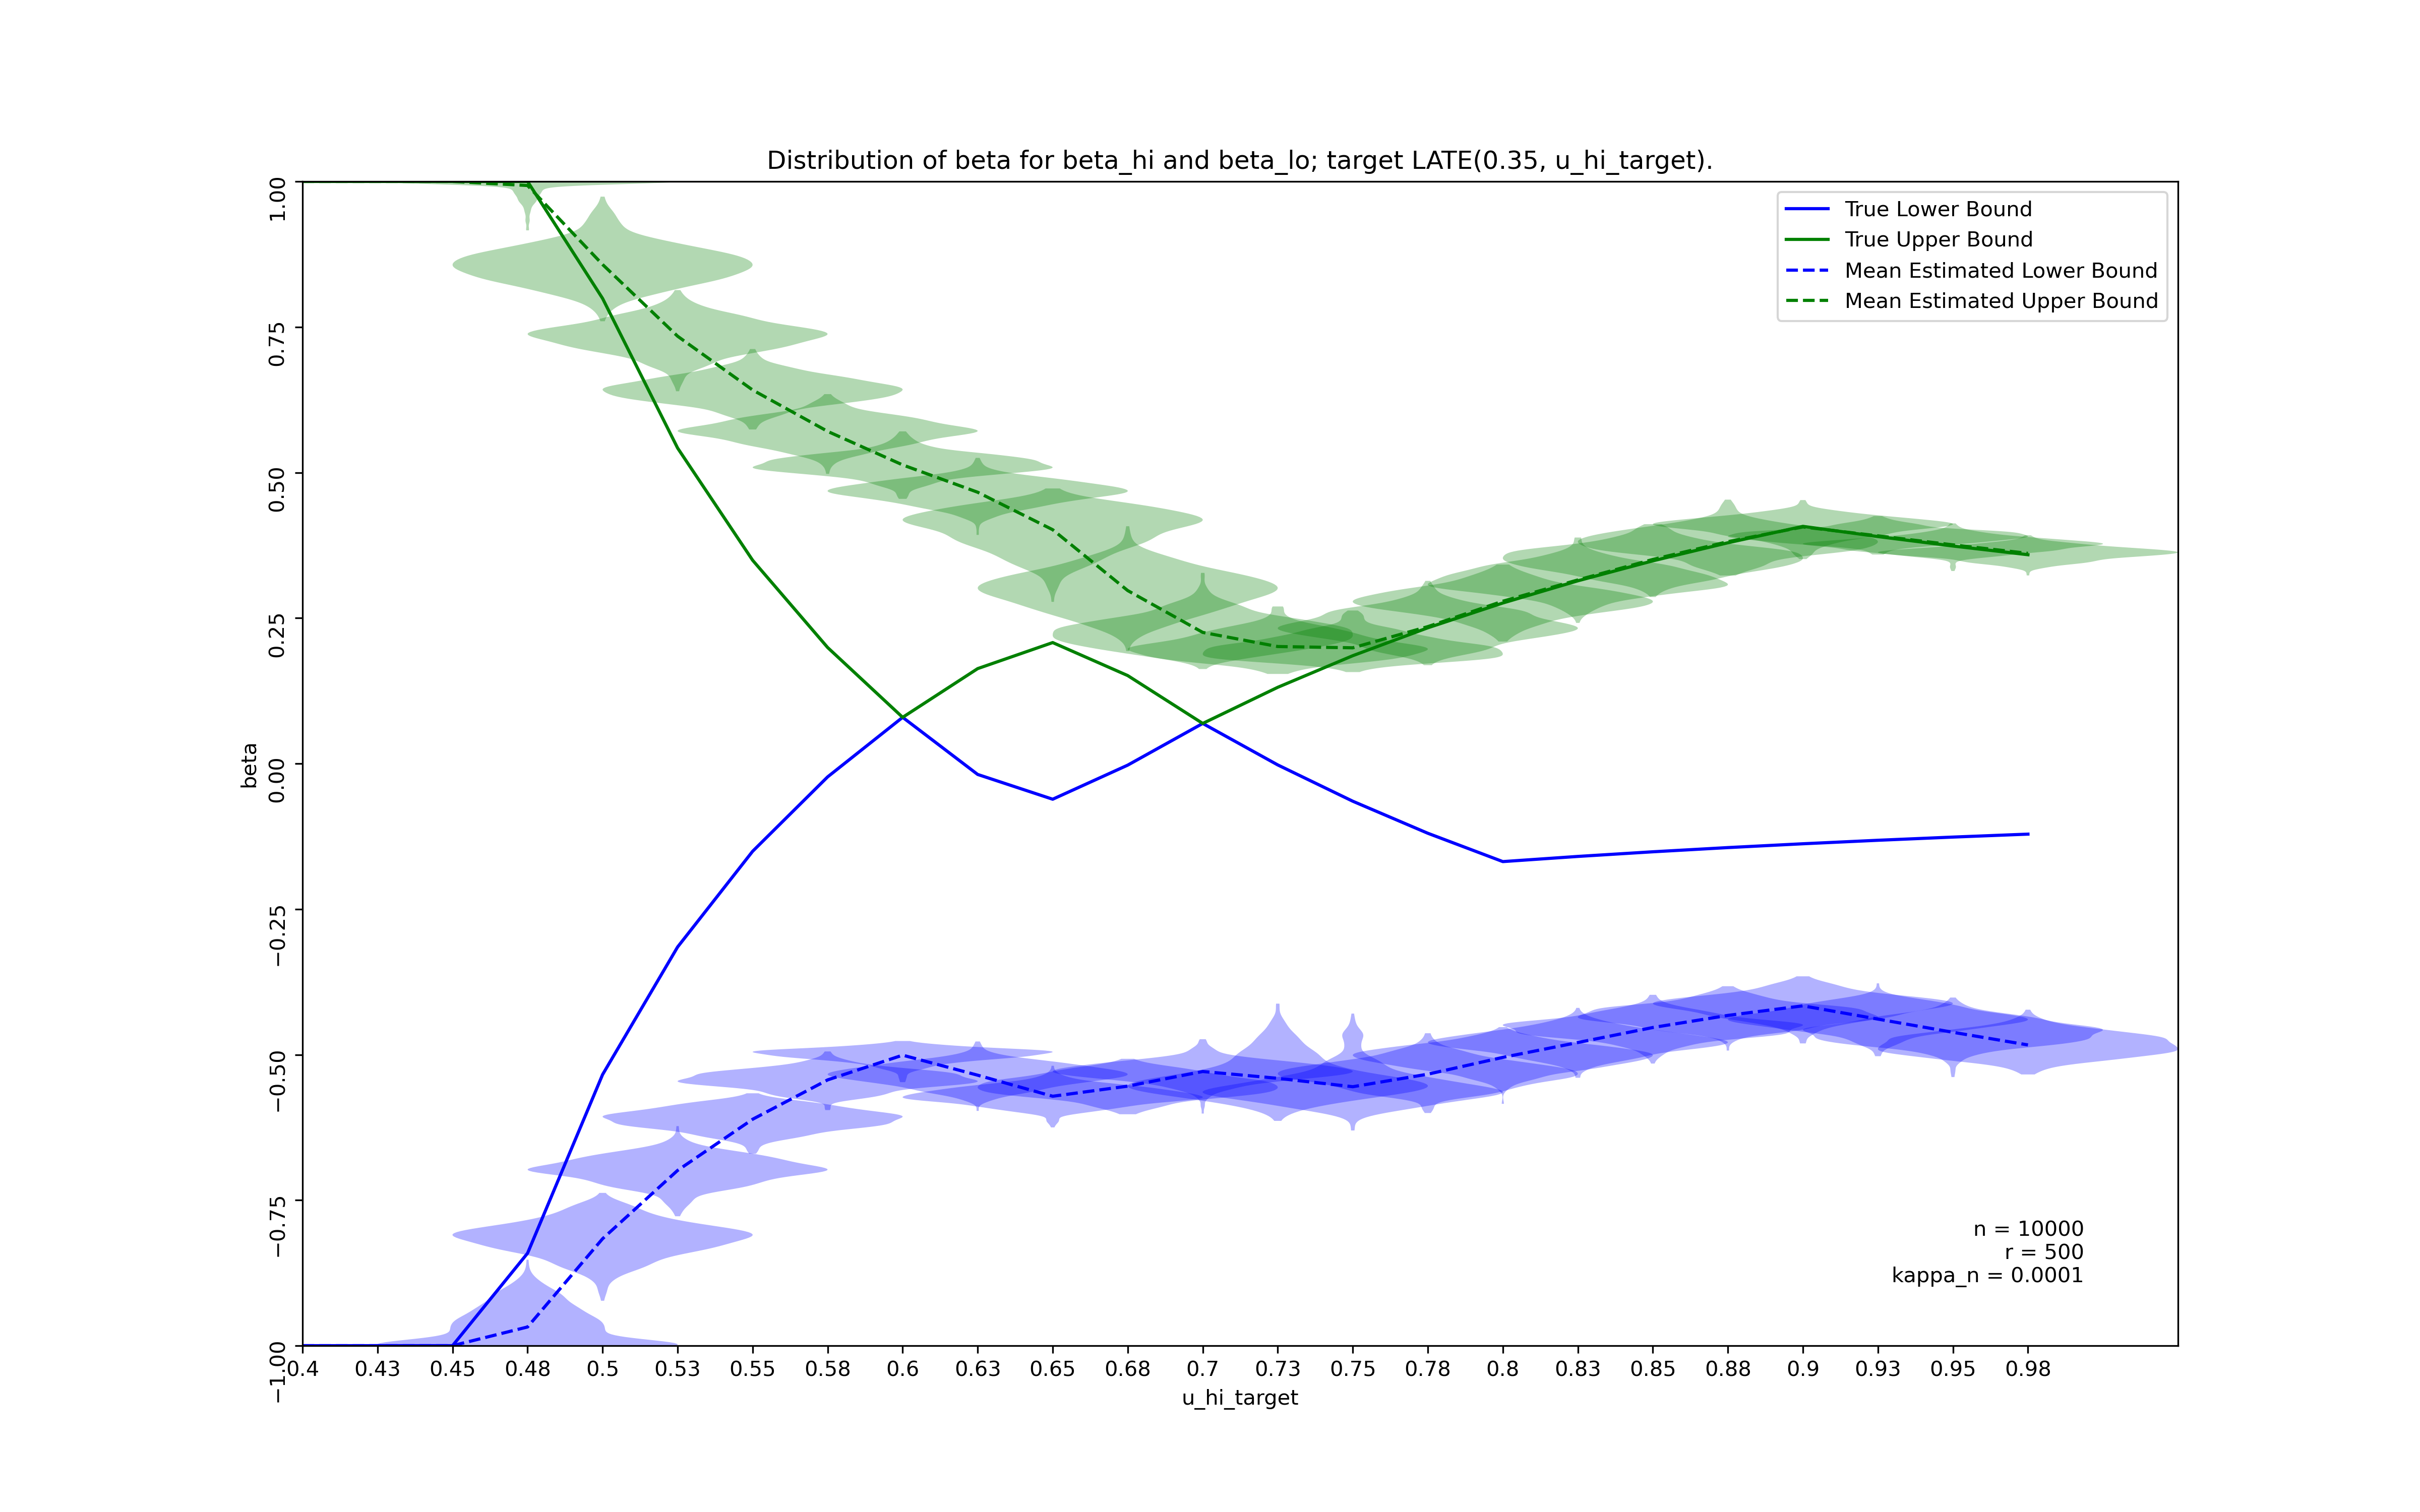
\includegraphics[width = \textwidth]{graph/simulation_sharp_bounds_10000_500_0.0001.png}
    \label{fig:main_sim_violin}
\end{figure}

\clearpage
\newpage

\section{Potential Future Analysis}
\begin{itemize}
    \item Weak IV
    \begin{itemize}
        \item Need to think about how this would be relevant; really weak IV is a failure of the regular asymptotic approximation to the finite sample distribution
        thereby making inference unreliable. This is not really an identification problem; i.e. for a discrete IV as long as not all propensity scores are the same we can always point identify some LATE.
        However, weak IV might show up in estimation of the bounds.
        \item Case of weak IV/many weak IV
        \item Weak IV for IV slope --> Use reduced form/cross-moments instead of IV-slope coefficient;
        thereby avoiding weak IV problem. Is this a trade-off between estimation and inference? I.e. identification bounds become wider
        but inference becomes more reliable?
    \end{itemize}
\end{itemize} 

\printbibliography

\appendix
\renewcommand\thefigure{\thesection.\arabic{figure}} 

\setcounter{table}{0}
\renewcommand{\thetable}{A\arabic{table}}

\clearpage
\newpage

\section{Choice of Tolerance}

\begin{figure}[h!]
    \caption{Simulation Results by Choice of $\kappa_n$ \label{app_fig:tolerances}}
     \centering

     \begin{subfigure}[b]{0.49\textwidth}
         \centering
          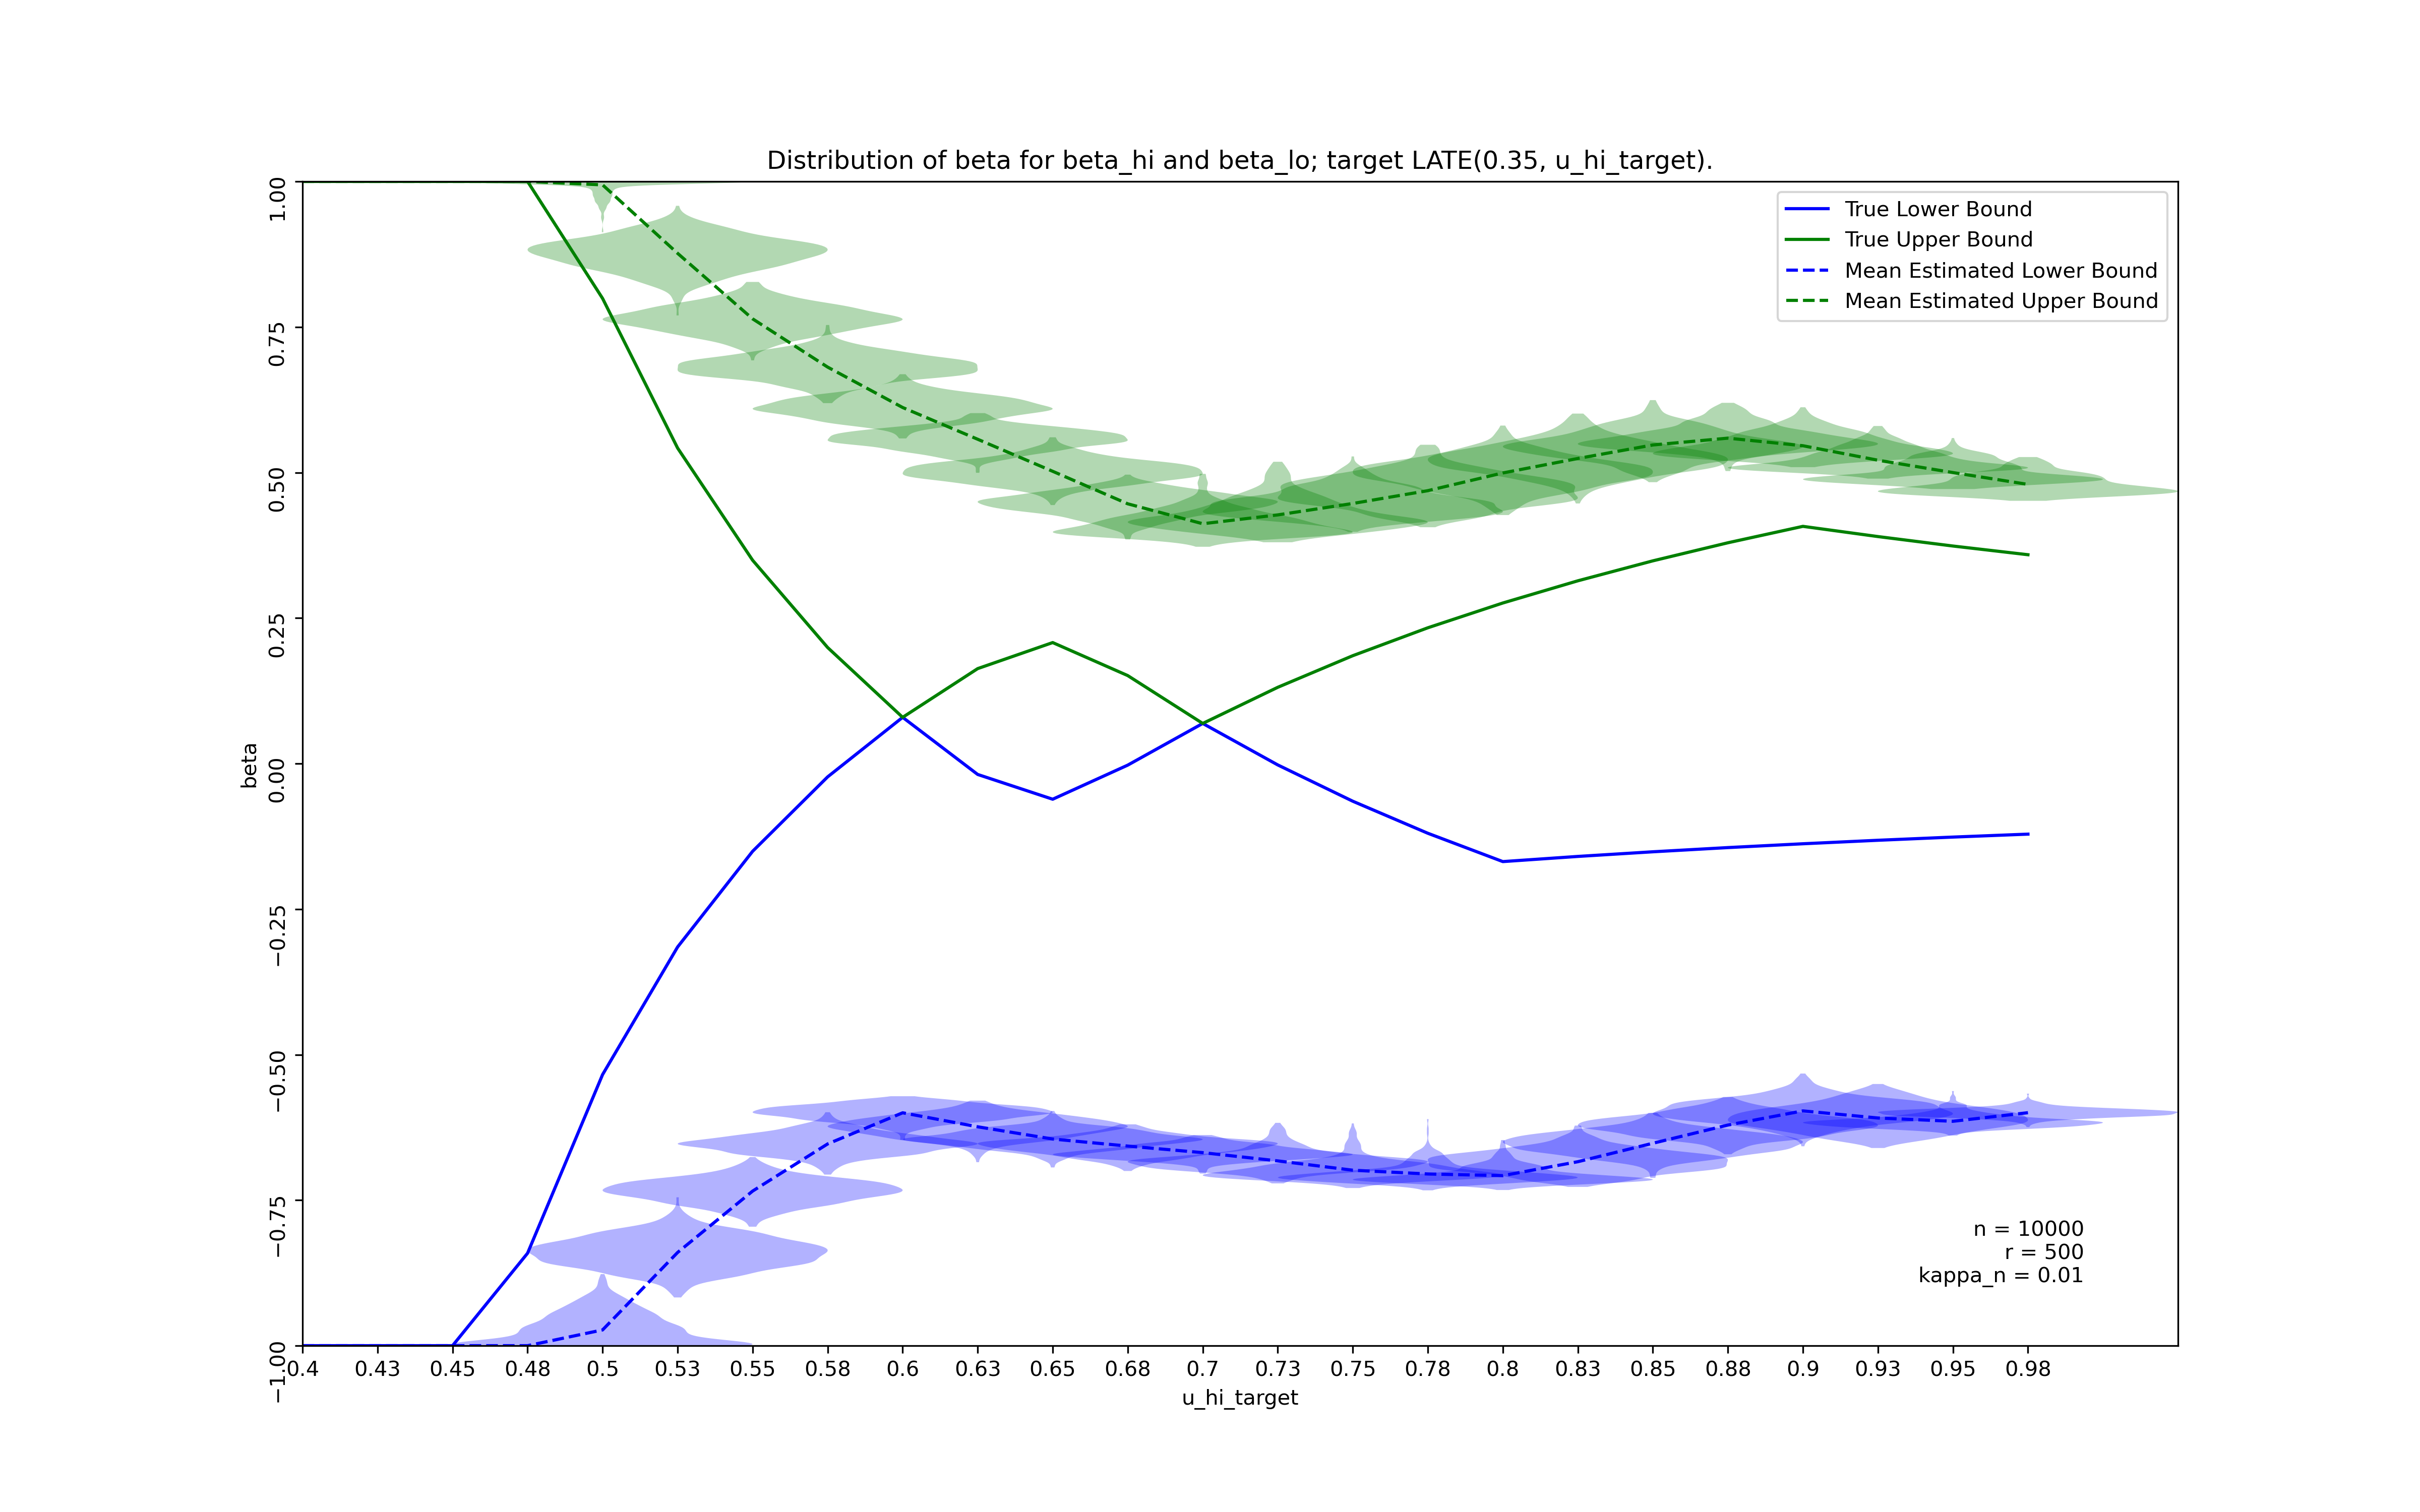
\includegraphics[width=\textwidth]{graph/simulation_sharp_bounds_10000_500_0.01}
         \subcaption{$\kappa_n = \frac{1}{\sqrt{n}}$}
     \end{subfigure}
    \hfill
     \begin{subfigure}[b]{0.49\textwidth}
         \centering
          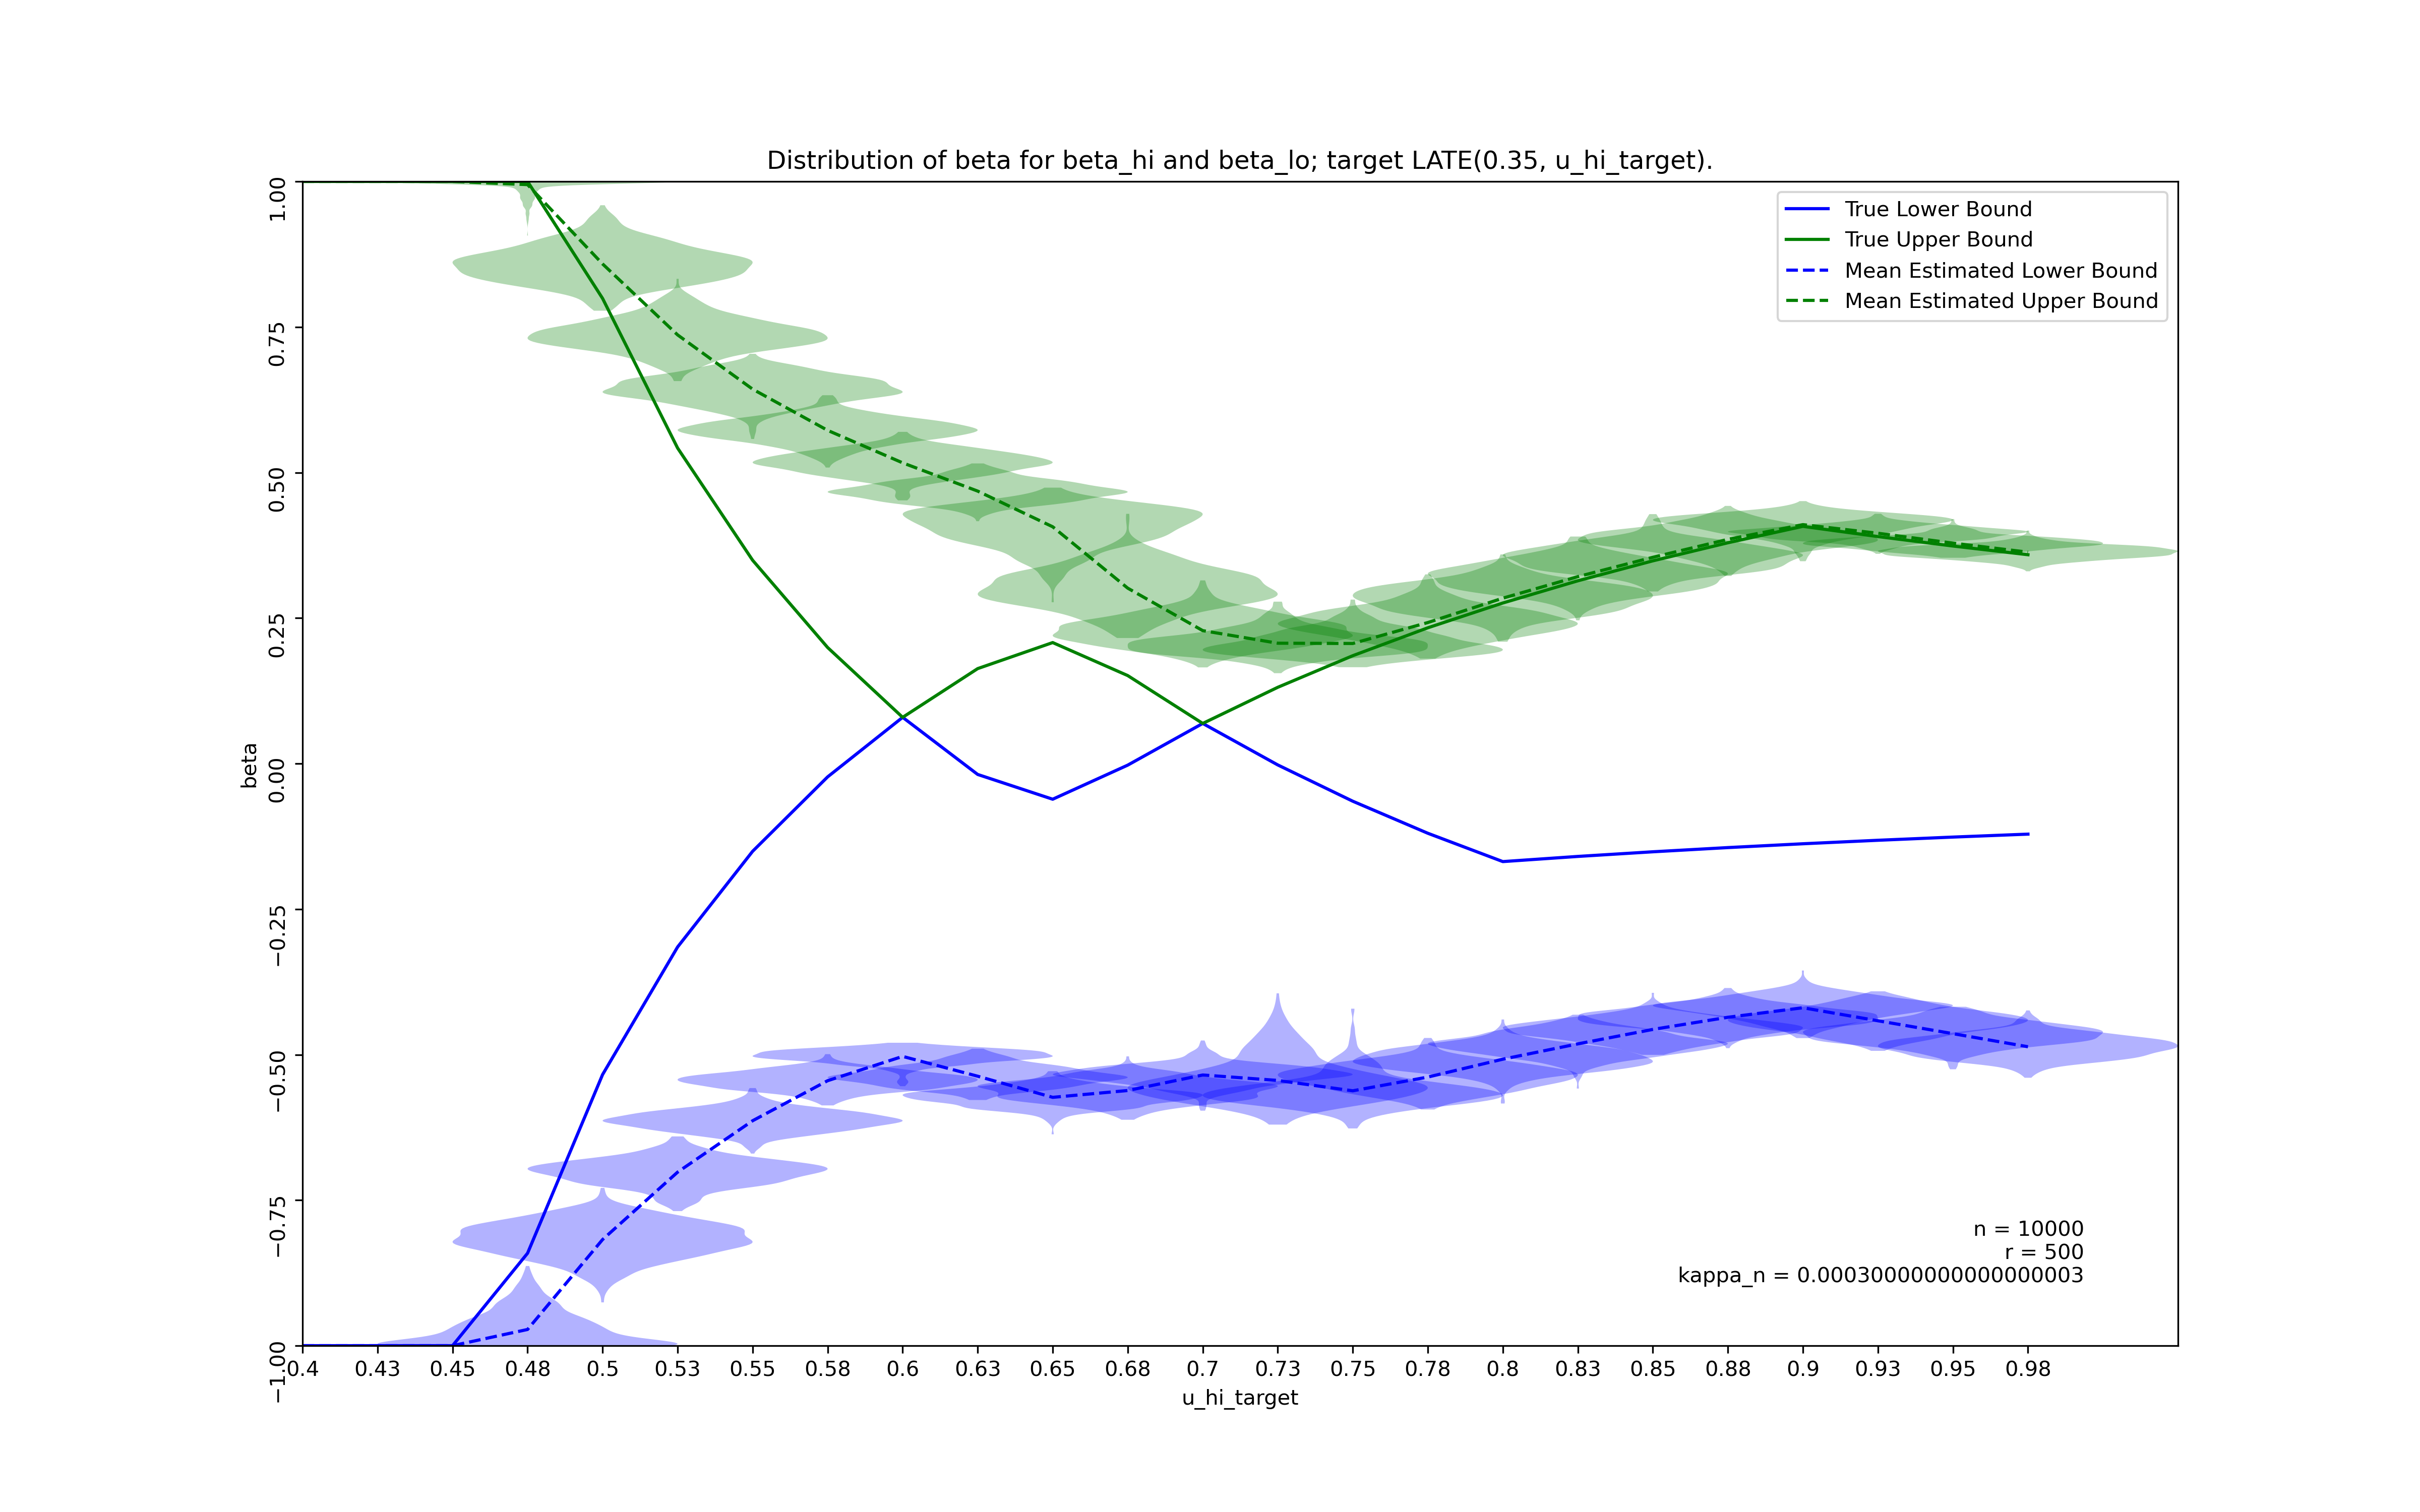
\includegraphics[width=\textwidth]{graph/simulation_sharp_bounds_10000_500_0.00030000000000000003.png}
          \subcaption{$\kappa_n = \frac{3}{n}$}
        \end{subfigure}

     \begin{subfigure}[b]{0.49\textwidth}
         \centering
         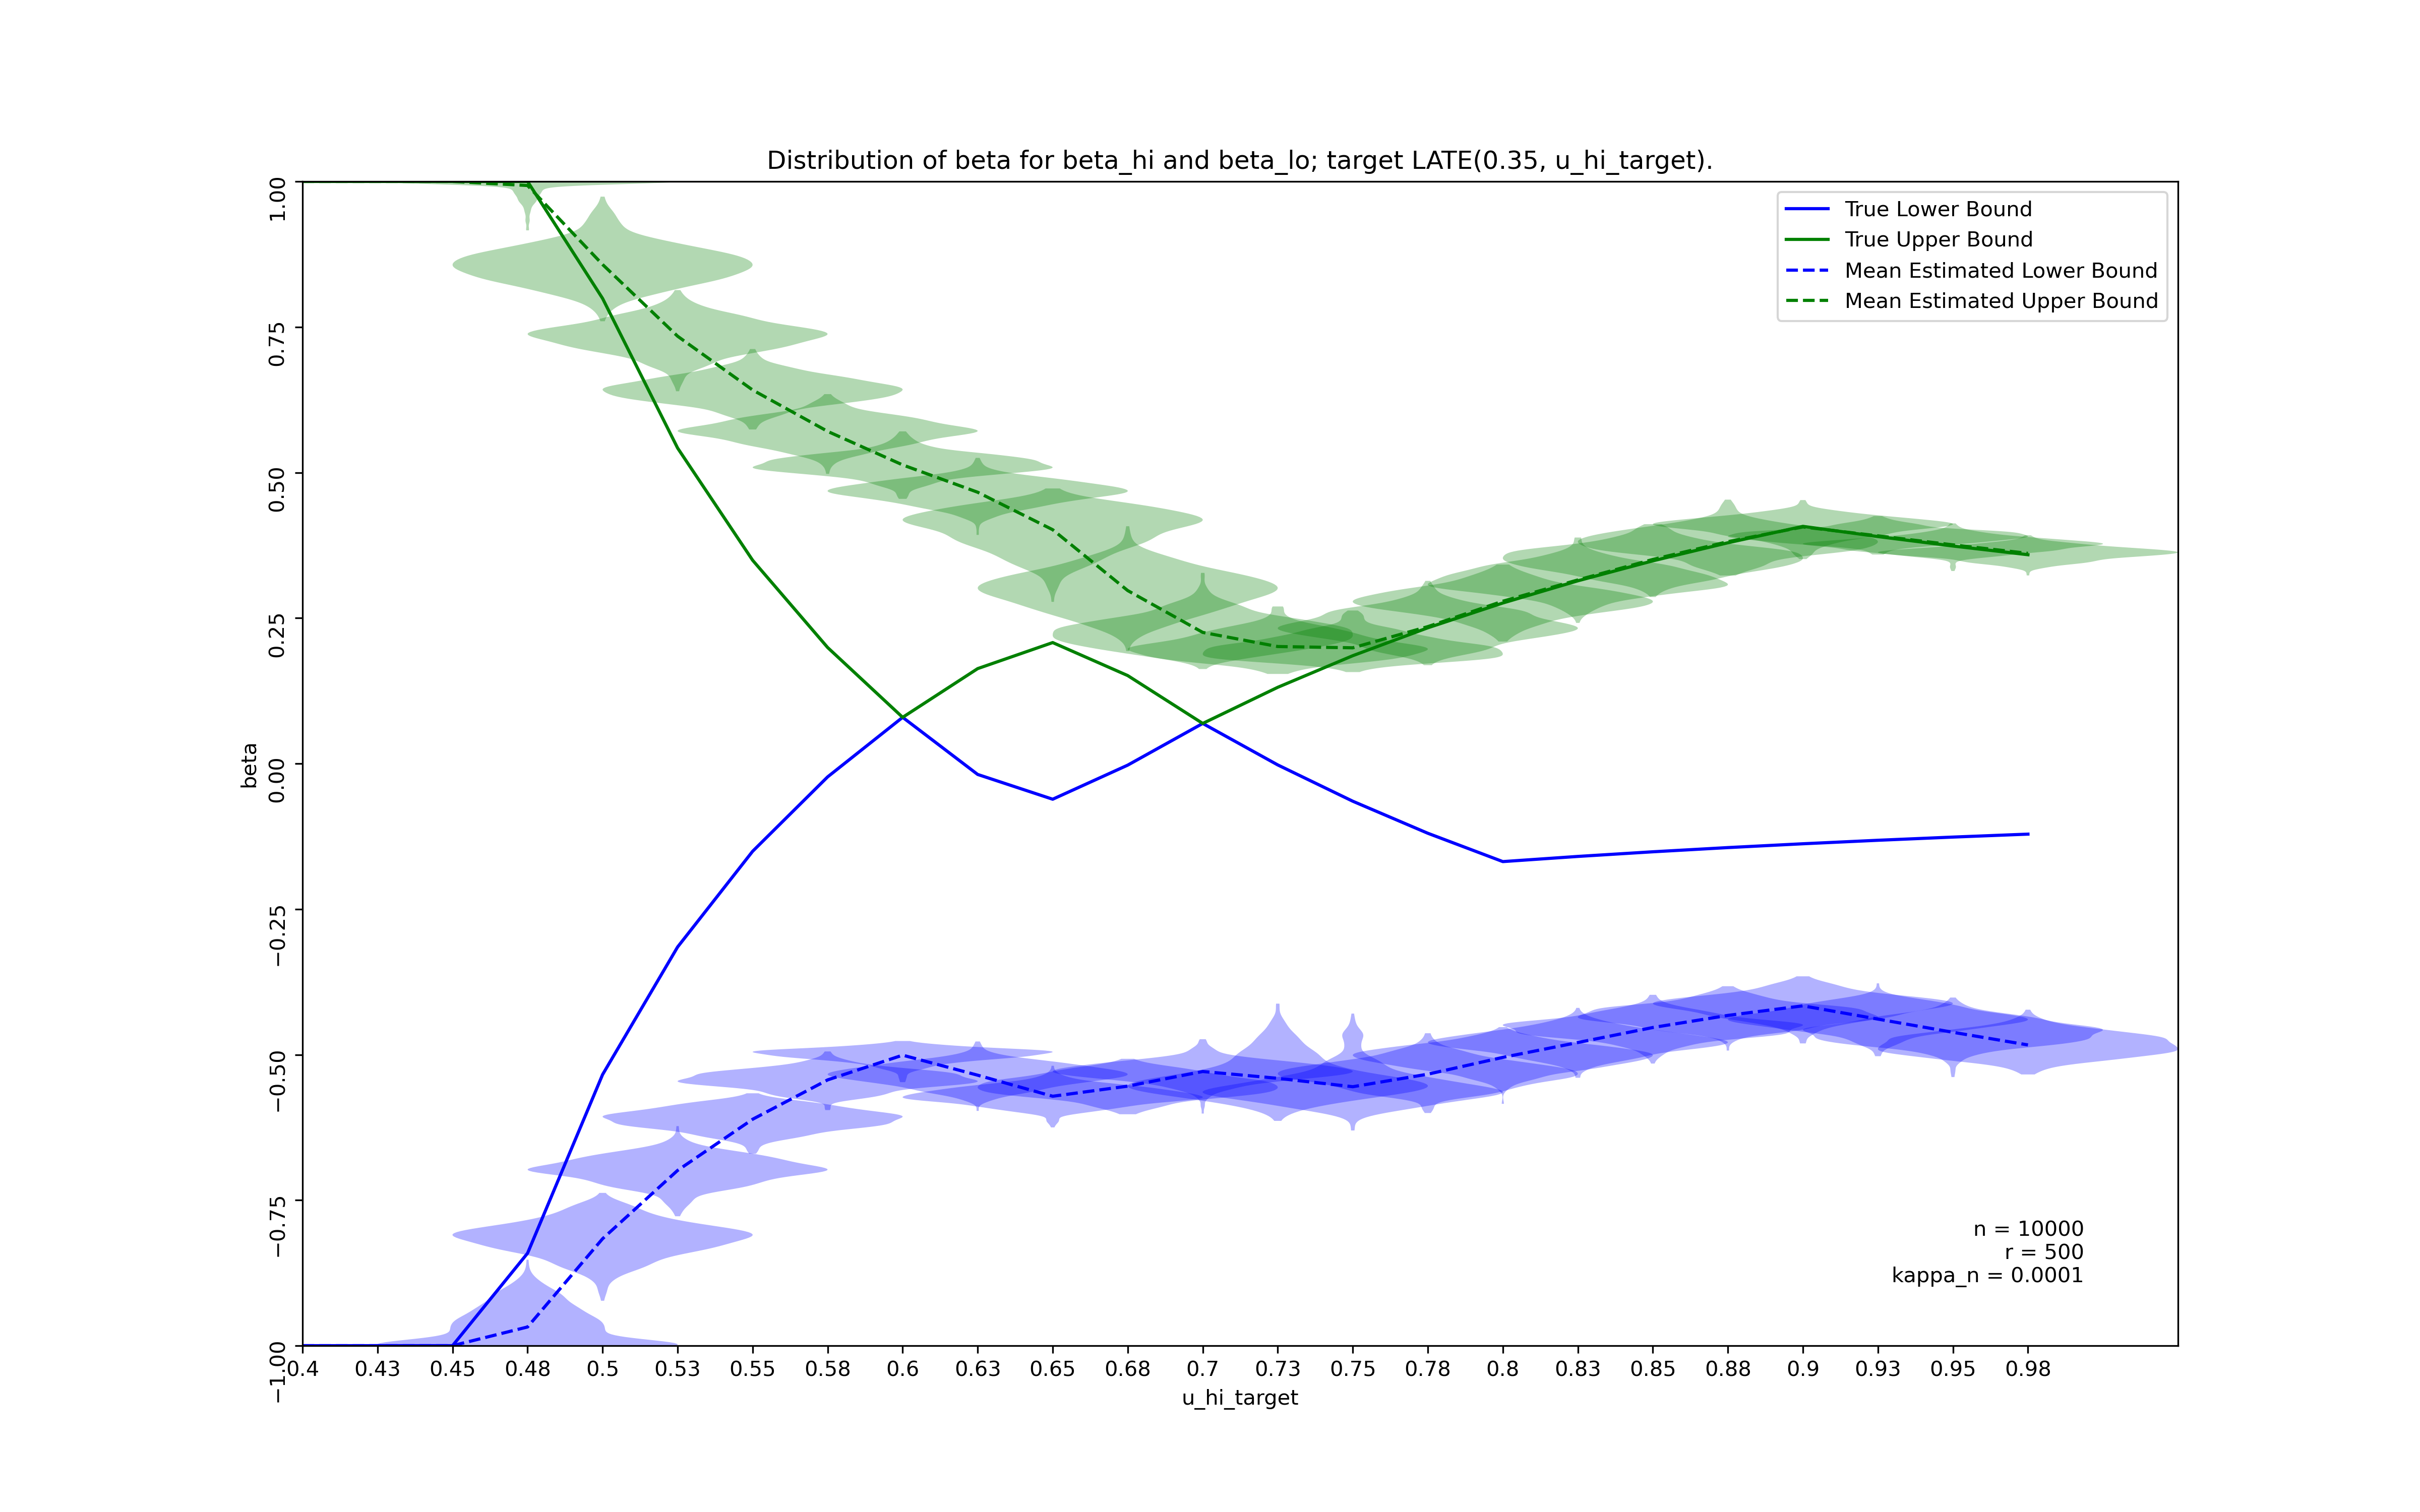
\includegraphics[width=\textwidth]{graph/simulation_sharp_bounds_10000_500_0.0001}
         \subcaption{$\kappa_n = \frac{1}{n}$}
     \end{subfigure}
    \hfill
     \begin{subfigure}[b]{0.49\textwidth}
         \centering
         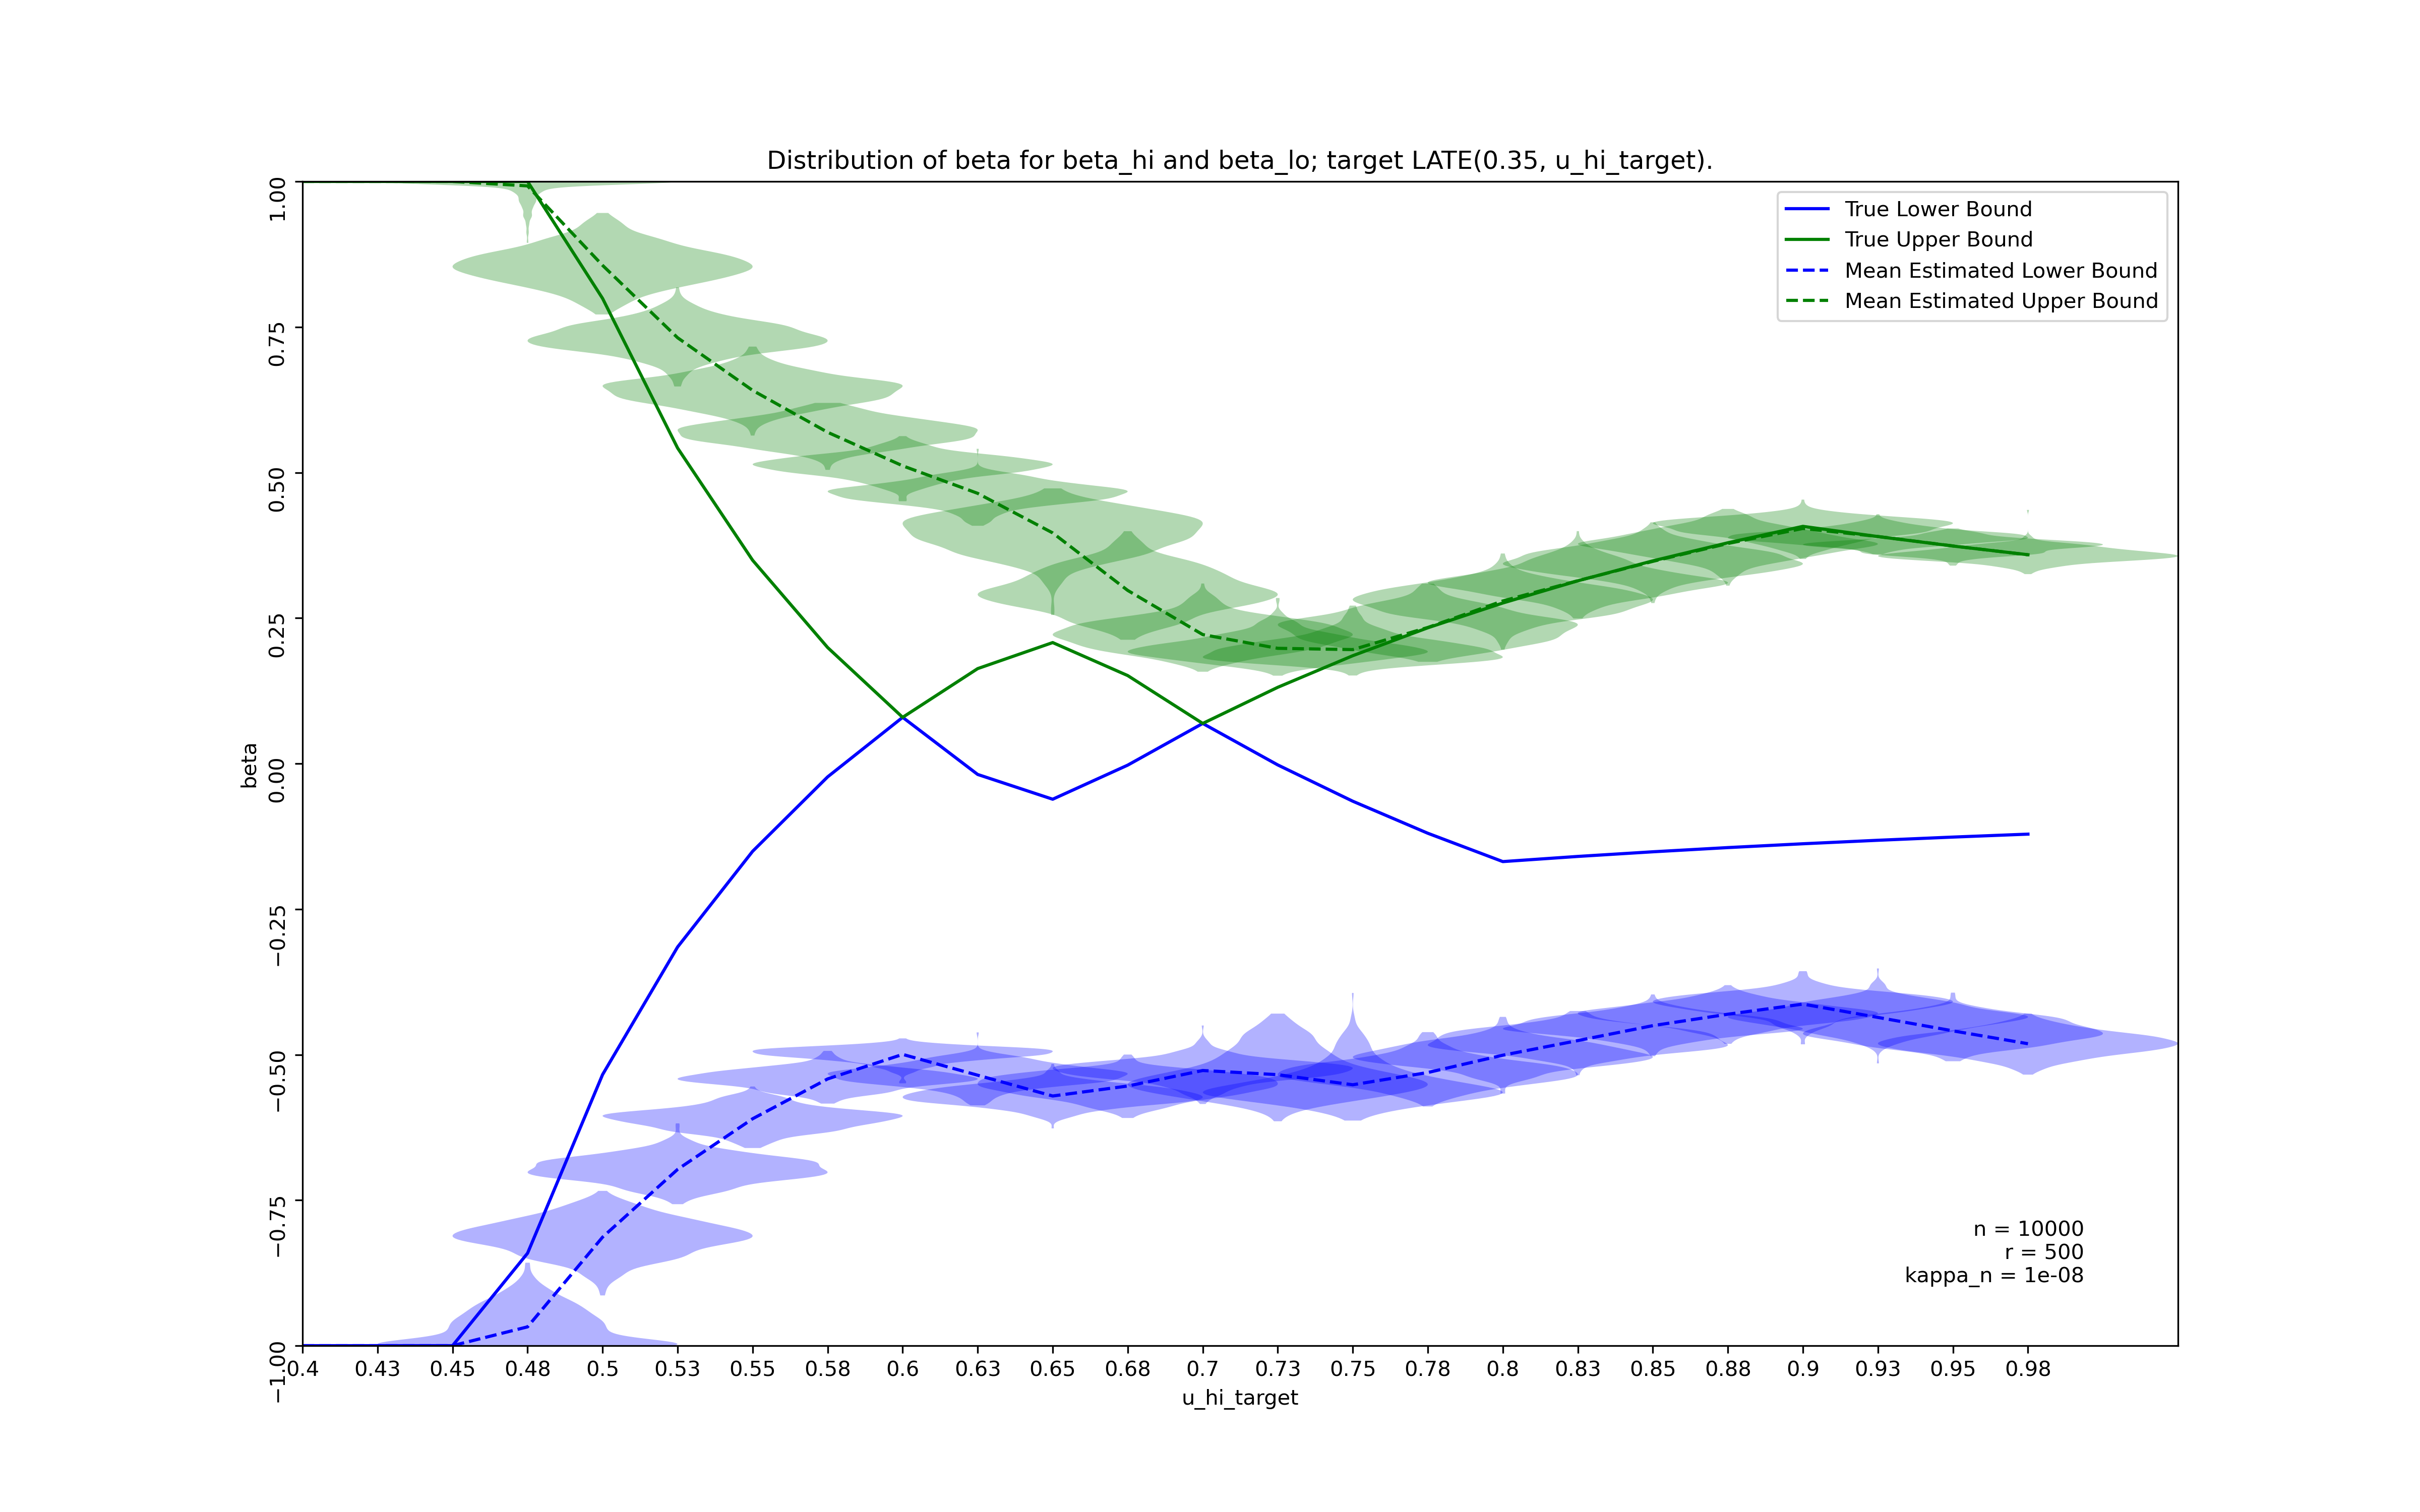
\includegraphics[width=\textwidth]{graph/simulation_sharp_bounds_10000_500_1e-08.png}
         \subcaption{$\kappa_n = \frac{1}{n^2}$}
     \end{subfigure}     
   
\floatfoot{\footnotesize

\textbf{Notes}: This figure compares simulation results for the main specificaiton described in Section \ref{sec:4_sim} for different tolerances levels $\kappa_n$.}

\end{figure}
\clearpage
\newpage

\section{Results for Larger Samples}
\begin{figure}[h!]
    \caption{Simulation Results for Larger Sample Sizes \label{app_fig:large_n}}
     \centering

     \begin{subfigure}[b]{0.49\textwidth}
         \centering
          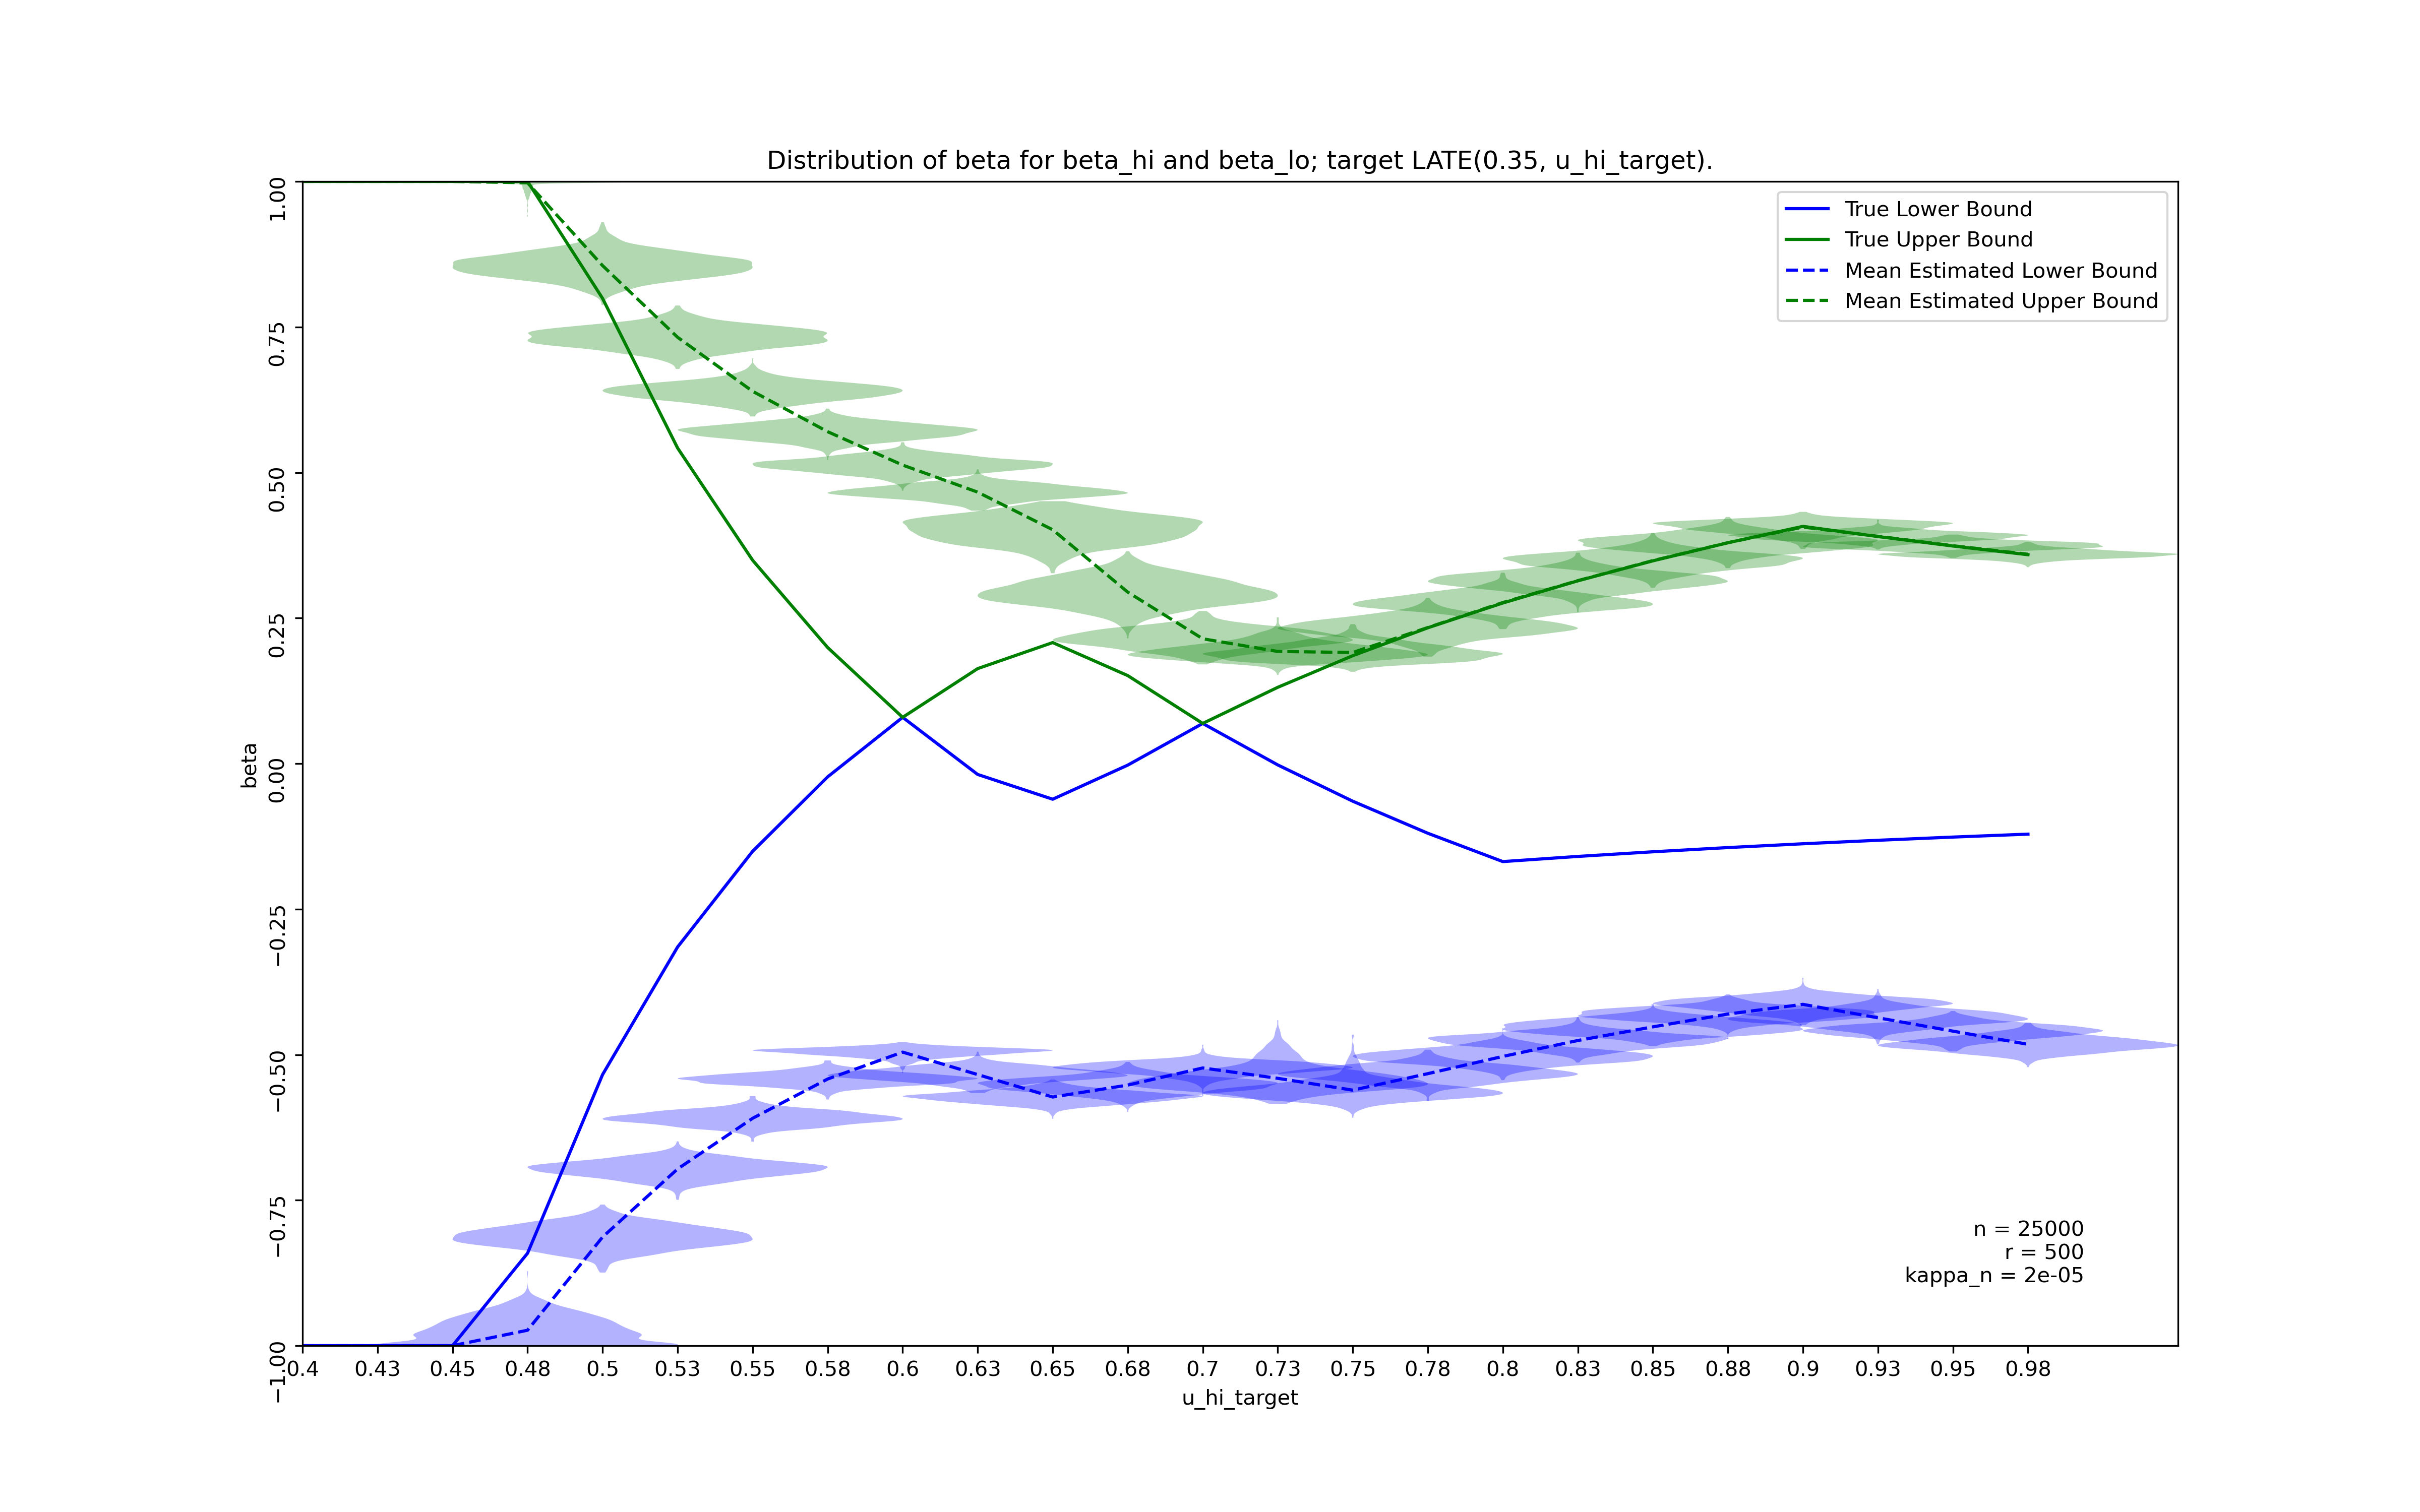
\includegraphics[width=\textwidth]{graph/simulation_sharp_bounds_25000_500_2e-05.png}
         \subcaption{$N=25,000$}
     \end{subfigure}
     \begin{subfigure}[b]{0.49\textwidth}
        \centering
        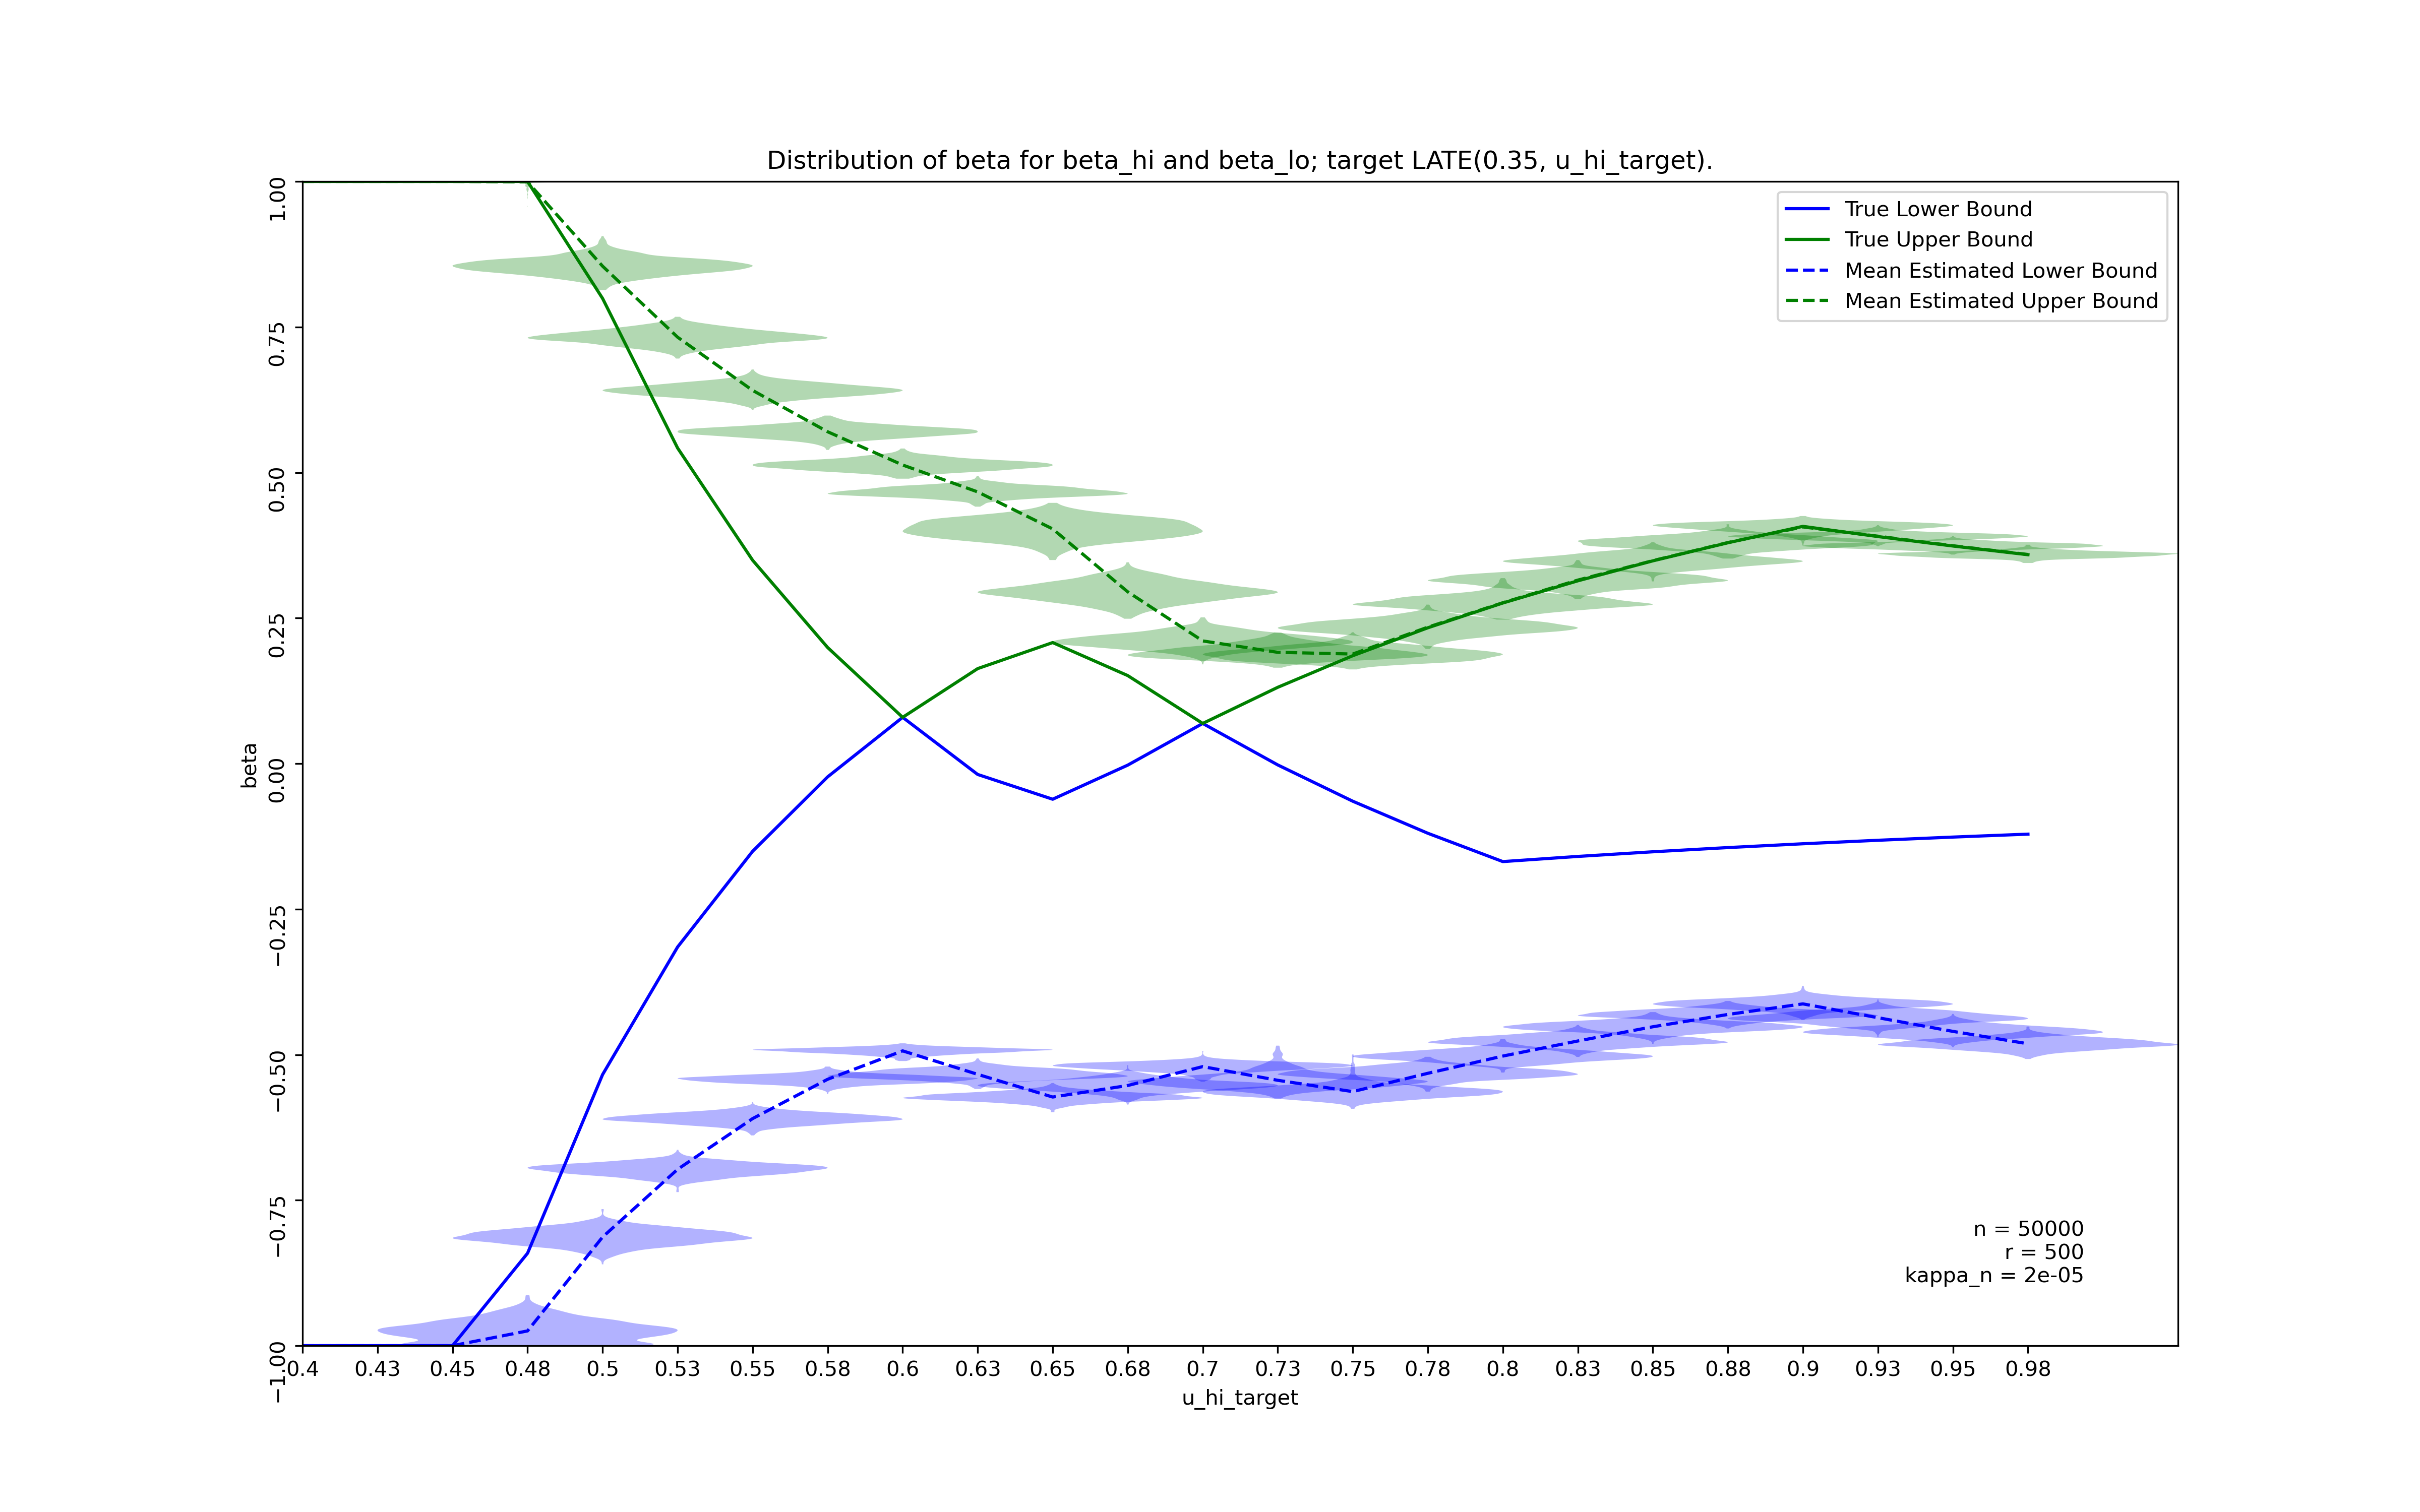
\includegraphics[width=\textwidth]{graph/simulation_sharp_bounds_50000_500_2e-05.png}
        \subcaption{$N=50,000$}
    \end{subfigure}
    
    \begin{subfigure}[b]{0.49\textwidth}
        \centering
         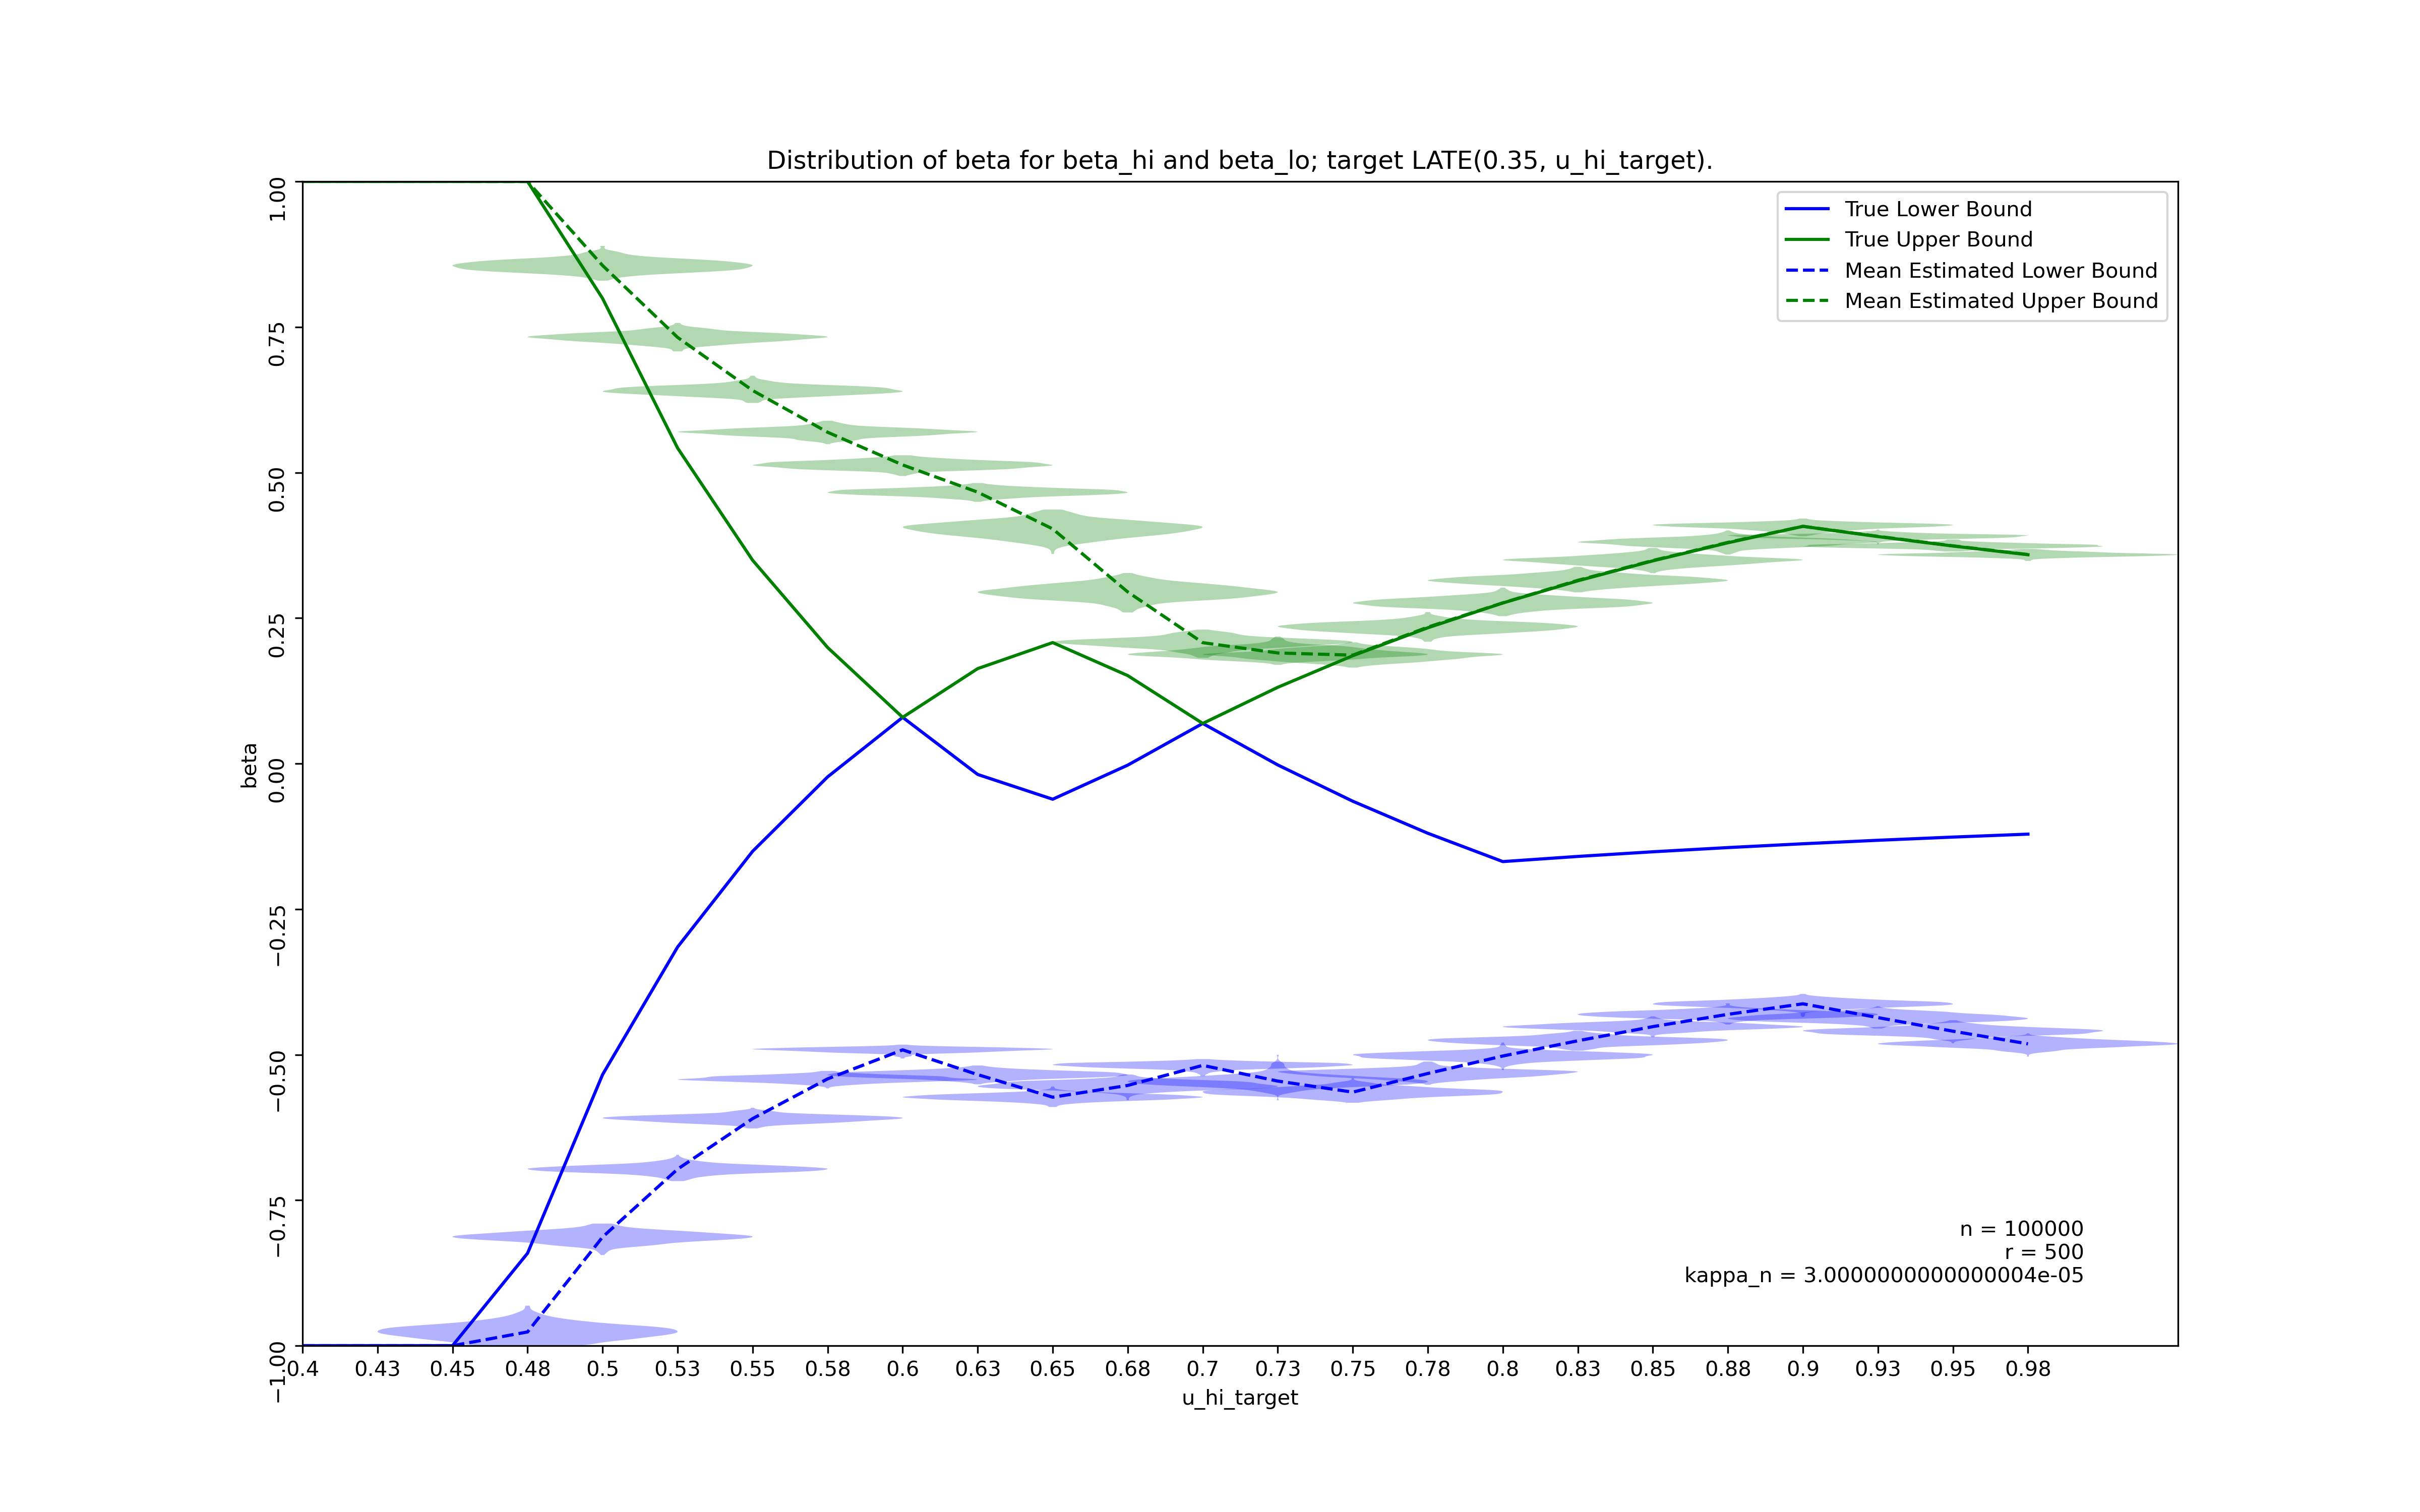
\includegraphics[width=\textwidth]{graph/simulation_sharp_bounds_100000_500_3.0000000000000004e-05.png}
        \subcaption{$N=100,000$}
    \end{subfigure}
   
\floatfoot{\footnotesize

\textbf{Notes}: This figure compares simulation results for the main specificaiton described in Section \ref{sec:4_sim} different samples sizes $N$.}

\end{figure}

\section{Unstable Estimator}

\begin{figure}
    \caption{Simulation Results: Bi-Modal Distribution \label{app_fig:bimodal}}
    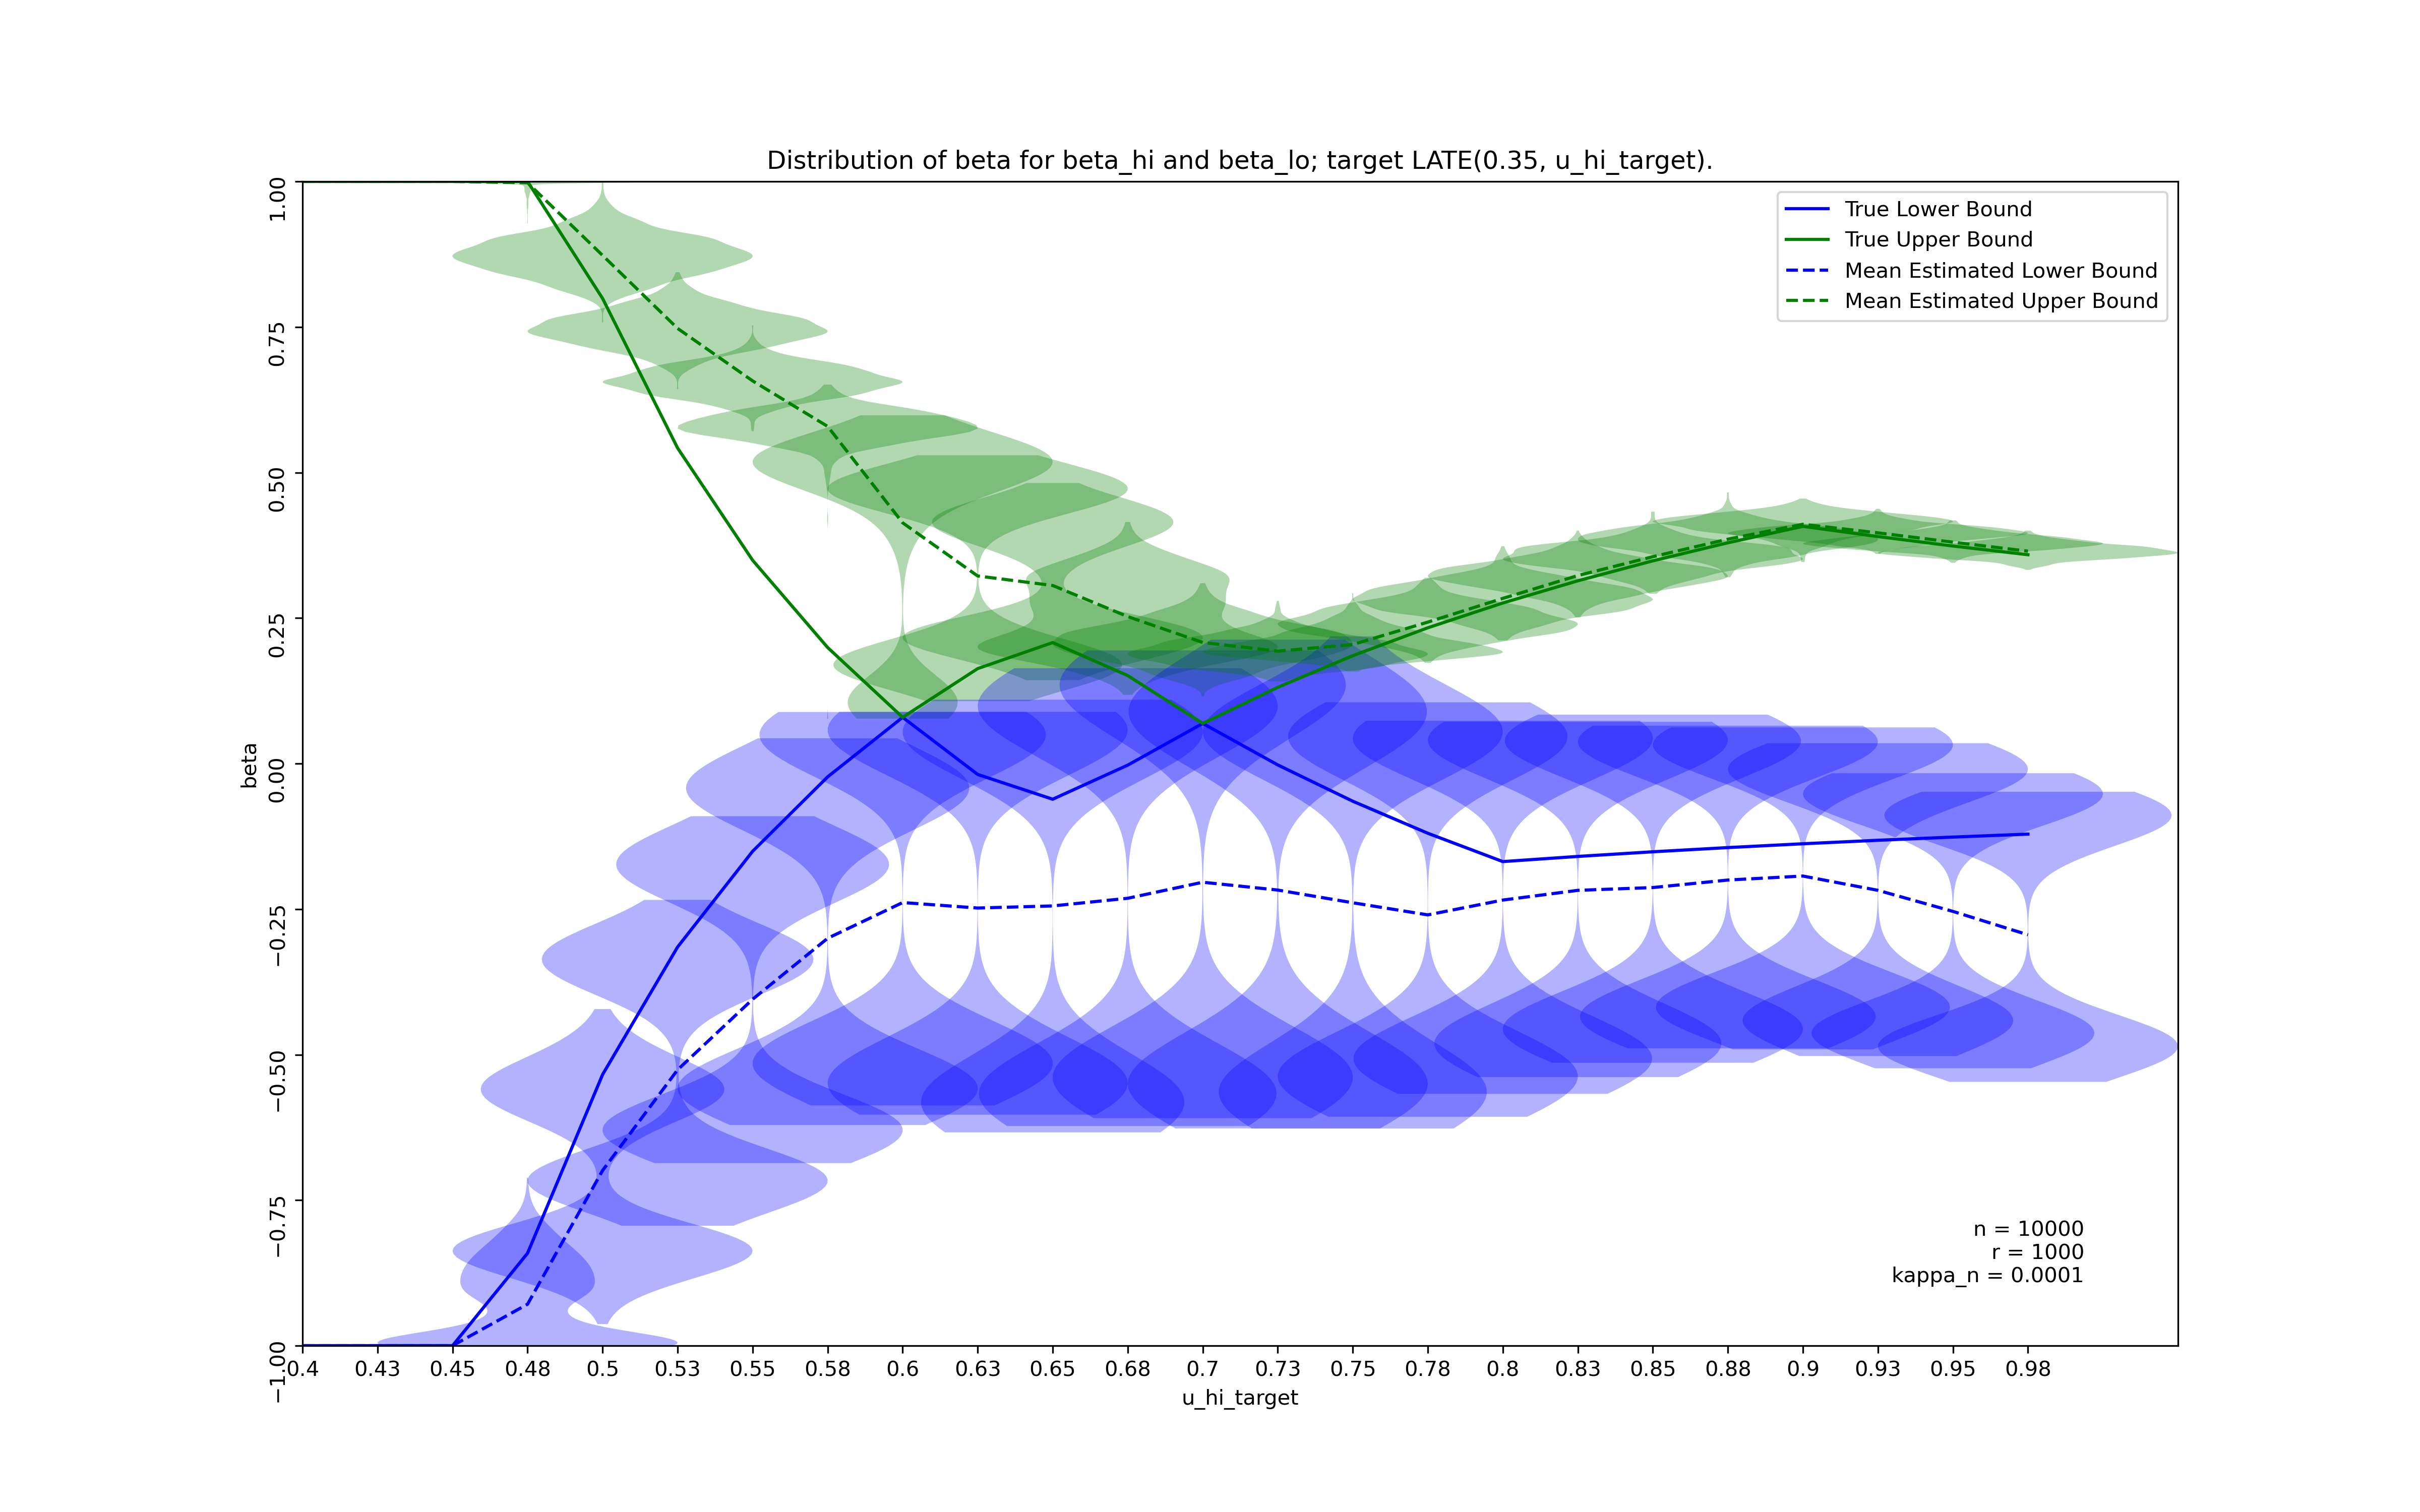
\includegraphics[width = \textwidth]{graph/simulation_sharp_bounds_unstable.png}

    \floatfoot{\footnotesize
    \textbf{Notes}: This figure shows results for the main specification when we use a partition including both estimated $\hat{p}(0)$ close to 0.35, and 0.35 in the partition for $u$.}

\end{figure}


\end{document}
